% Options for packages loaded elsewhere
\PassOptionsToPackage{unicode}{hyperref}
\PassOptionsToPackage{hyphens}{url}
%
\documentclass[
]{article}
\usepackage{amsmath,amssymb}
\usepackage{iftex}
\ifPDFTeX
  \usepackage[T1]{fontenc}
  \usepackage[utf8]{inputenc}
  \usepackage{textcomp} % provide euro and other symbols
\else % if luatex or xetex
  \usepackage{unicode-math} % this also loads fontspec
  \defaultfontfeatures{Scale=MatchLowercase}
  \defaultfontfeatures[\rmfamily]{Ligatures=TeX,Scale=1}
\fi
\usepackage{lmodern}
\ifPDFTeX\else
  % xetex/luatex font selection
\fi
% Use upquote if available, for straight quotes in verbatim environments
\IfFileExists{upquote.sty}{\usepackage{upquote}}{}
\IfFileExists{microtype.sty}{% use microtype if available
  \usepackage[]{microtype}
  \UseMicrotypeSet[protrusion]{basicmath} % disable protrusion for tt fonts
}{}
\makeatletter
\@ifundefined{KOMAClassName}{% if non-KOMA class
  \IfFileExists{parskip.sty}{%
    \usepackage{parskip}
  }{% else
    \setlength{\parindent}{0pt}
    \setlength{\parskip}{6pt plus 2pt minus 1pt}}
}{% if KOMA class
  \KOMAoptions{parskip=half}}
\makeatother
\usepackage{xcolor}
\usepackage[margin=1in]{geometry}
\usepackage{longtable,booktabs,array}
\usepackage{calc} % for calculating minipage widths
% Correct order of tables after \paragraph or \subparagraph
\usepackage{etoolbox}
\makeatletter
\patchcmd\longtable{\par}{\if@noskipsec\mbox{}\fi\par}{}{}
\makeatother
% Allow footnotes in longtable head/foot
\IfFileExists{footnotehyper.sty}{\usepackage{footnotehyper}}{\usepackage{footnote}}
\makesavenoteenv{longtable}
\usepackage{graphicx}
\makeatletter
\def\maxwidth{\ifdim\Gin@nat@width>\linewidth\linewidth\else\Gin@nat@width\fi}
\def\maxheight{\ifdim\Gin@nat@height>\textheight\textheight\else\Gin@nat@height\fi}
\makeatother
% Scale images if necessary, so that they will not overflow the page
% margins by default, and it is still possible to overwrite the defaults
% using explicit options in \includegraphics[width, height, ...]{}
\setkeys{Gin}{width=\maxwidth,height=\maxheight,keepaspectratio}
% Set default figure placement to htbp
\makeatletter
\def\fps@figure{htbp}
\makeatother
\setlength{\emergencystretch}{3em} % prevent overfull lines
\providecommand{\tightlist}{%
  \setlength{\itemsep}{0pt}\setlength{\parskip}{0pt}}
\setcounter{secnumdepth}{-\maxdimen} % remove section numbering
\ifLuaTeX
  \usepackage{selnolig}  % disable illegal ligatures
\fi
\IfFileExists{bookmark.sty}{\usepackage{bookmark}}{\usepackage{hyperref}}
\IfFileExists{xurl.sty}{\usepackage{xurl}}{} % add URL line breaks if available
\urlstyle{same}
\hypersetup{
  hidelinks,
  pdfcreator={LaTeX via pandoc}}

\author{}
\date{\vspace{-2.5em}}

\begin{document}

\hypertarget{guuxeda-de-matemuxe1ticas-iii-otouxf1o-2023}{%
\section{Guía de Matemáticas III, Otoño
2023}\label{guuxeda-de-matemuxe1ticas-iii-otouxf1o-2023}}

\hypertarget{primer-parcial}{%
\subsection{Primer Parcial}\label{primer-parcial}}

\hypertarget{operaciones-con-matrices}{%
\subsubsection{Operaciones con
matrices}\label{operaciones-con-matrices}}

\hypertarget{sea-a-beginpmatrix-1-1-3-5-2-6--2--1--3endpmatrix-aproxime-cos2a-con-una-serie-de-maclaurin}{%
\paragraph{\texorpdfstring{1. Sea
\(A = \begin{pmatrix} 1 & 1 & 3 \\ 5 & 2 & 6\\ -2 & -1& -3\end{pmatrix}\),
aproxime \(\cos{2A}\) con una serie de
Maclaurin}{1. Sea A = \textbackslash begin\{pmatrix\} 1 \& 1 \& 3 \textbackslash\textbackslash{} 5 \& 2 \& 6\textbackslash\textbackslash{} -2 \& -1\& -3\textbackslash end\{pmatrix\}, aproxime \textbackslash cos\{2A\} con una serie de Maclaurin}}\label{sea-a-beginpmatrix-1-1-3-5-2-6--2--1--3endpmatrix-aproxime-cos2a-con-una-serie-de-maclaurin}}

\[
2A = \begin{pmatrix}
    2 & 2 & 6 \\
    10 & 4 & 12 \\
    -4 & -2 & -6
\end{pmatrix} \\
\]

\[
A^2 = A\times A =
\begin{pmatrix}
2 & 2 & 6 \\
10 & 4 & 12 \\
-4& -2 &-6
\end {pmatrix} \times \begin{pmatrix}
2 & 2 & 6 \\
10 & 4 & 12 \\
-4& -2 &-6
\end {pmatrix} = \begin{pmatrix}
0&0&0&\\12&12&36\\-4&-4&-12
\end {pmatrix}
\]

\[
A^4 = A^2\times A^2 = \begin{pmatrix}
0&0&0&\\12&12&36\\-4&-4&-12
\end {pmatrix} \times \begin{pmatrix}
0&0&0&\\12&12&36\\-4&-4&-12
\end {pmatrix} = \begin{pmatrix}
0&0&0\\0&0&0&\\0&0&0&\end {pmatrix}
\]

\[
A^6 = A^4 \times A^2 = \begin{pmatrix}
0&0&0\\0&0&0&\\0&0&0&\end {pmatrix} \times \begin{pmatrix}
0&0&0&\\12&12&36\\-4&-4&-12
\end {pmatrix} = \begin{pmatrix}
0&0&0\\0&0&0\\0&0&0
\end {pmatrix}
\]

\[
cos(2A) = 1 - \frac{2A^2}{2!} + \frac{2A^4}{4!} - \frac{2A^6}{6!} = 1 - \frac{2\left(\begin{pmatrix}
0&0&0&\\12&12&36\\-4&-4&-12
\end {pmatrix}\right)}{2!} + \frac{2\left(\begin{pmatrix}
0&0&0\\0&0&0&\\0&0&0&\end {pmatrix}\right)}{4!} - \frac{2\left(\begin{pmatrix}
0&0&0\\0&0&0\\0&0&0
\end {pmatrix}\right)}{6!} \\= 1-\left(\begin{pmatrix}
0&0&0\\6&6&18\\-2&-2&-6\end{pmatrix} + \begin{pmatrix}
0&0&0\\0&0&0\\0&0&0\end {pmatrix}+ \begin{pmatrix}
0&0&0\\0&0&0\\0&0&0\end {pmatrix}\right) \\ = 1- \begin{pmatrix} 0&0&0\\6&6&18\\-2&-2&-6\end{pmatrix}
\]

\hypertarget{sea-a-beginpmatrix--1-2-21-x-0231endpmatrix-y-b-beginpmatrix3-110-31-20x-endpmatrix.-cuuxe1l-es-el-valor-de-x-para-que-trazaa-3i_3bt-13}{%
\paragraph{\texorpdfstring{2. Sea
\(A = \begin{pmatrix} -1 & 2& 2&\\1 & x & 0\\2&3&1\end{pmatrix}\) y
\(B = \begin{pmatrix}3&-1&1\\0&-3&1\\-2&0&x \end{pmatrix}\). ¿Cuál es el
valor de \(x\) para que
\(Traza(A-3I_3+B^T) = 13\)?}{2. Sea A = \textbackslash begin\{pmatrix\} -1 \& 2\& 2\&\textbackslash\textbackslash1 \& x \& 0\textbackslash\textbackslash2\&3\&1\textbackslash end\{pmatrix\} y B = \textbackslash begin\{pmatrix\}3\&-1\&1\textbackslash\textbackslash0\&-3\&1\textbackslash\textbackslash-2\&0\&x \textbackslash end\{pmatrix\}. ¿Cuál es el valor de x para que Traza(A-3I\_3+B\^{}T) = 13?}}\label{sea-a-beginpmatrix--1-2-21-x-0231endpmatrix-y-b-beginpmatrix3-110-31-20x-endpmatrix.-cuuxe1l-es-el-valor-de-x-para-que-trazaa-3i_3bt-13}}

\[
I_3 =  \begin{pmatrix}1&0&0\\0&1&0\\0&0&1\end{pmatrix}
\]

\[
A-3I_3+B^T =  \begin{pmatrix} -1 & 2& 2&\\1 & x & 0\\2&3&1\end{pmatrix} -  3\begin{pmatrix}1&0&0\\0&1&0\\0&0&\end{pmatrix} +  \begin{pmatrix}3&0&-2\\-1&-3&0\\1&1&x\end{pmatrix} =  \begin{pmatrix}-1&2&0\\0&x-6&0\\3&4&x-2\end{pmatrix}
\]

\[
Traza(\begin{pmatrix}-1&2&0\\0&x-6&0\\3&4&x-2\end{pmatrix}) \rightarrow \begin{align*}
    -1+x+6+x-2 = 13\\
    2x-9=13\\
    2x=22\\
    x = 11
\end{align*}
\]

\hypertarget{dada-la-matriz-a-beginpmatrix--1720-58-endpmatrix-determine-una-matrix-b-yal-que-ba-beginpmatrix--3-9-0-4-0-1-endpmatrix}{%
\paragraph{\texorpdfstring{3. Dada la matriz
\(A= \begin{pmatrix} -1&7&2\\0&-5&8 \end{pmatrix}\), determine una
matrix \(B\) yal que
\(BA = \begin{pmatrix} -3 & 9 & 0 \\ 4 & 0 & 1 \end{pmatrix}\)}{3. Dada la matriz A= \textbackslash begin\{pmatrix\} -1\&7\&2\textbackslash\textbackslash0\&-5\&8 \textbackslash end\{pmatrix\}, determine una matrix B yal que BA = \textbackslash begin\{pmatrix\} -3 \& 9 \& 0 \textbackslash\textbackslash{} 4 \& 0 \& 1 \textbackslash end\{pmatrix\}}}\label{dada-la-matriz-a-beginpmatrix--1720-58-endpmatrix-determine-una-matrix-b-yal-que-ba-beginpmatrix--3-9-0-4-0-1-endpmatrix}}

\[
B = (BA)A^{-1} =  \begin{pmatrix} -3 & 9 & 0 \\ 4 & 0 & 1 \end{pmatrix}
\]

\hypertarget{encuentre-las-matrices-a-y-b-que-resuelven-el-sistema-begincases-2a-b-beginpmatrix-1--4-6-0-endpmatrix-a--3b-beginpmatrix--2-1-3--4-endpmatrix-endcases}{%
\paragraph{\texorpdfstring{4. Encuentre las matrices \(A\) y \(B\) que
resuelven el sistema
\(\begin{cases} 2A + B = \begin{pmatrix} 1 & -4 \\ 6 & 0 \end{pmatrix} \\ A -3B = \begin{pmatrix} -2 & 1 \\ 3 & -4 \end{pmatrix} \end{cases}\)}{4. Encuentre las matrices A y B que resuelven el sistema \textbackslash begin\{cases\} 2A + B = \textbackslash begin\{pmatrix\} 1 \& -4 \textbackslash\textbackslash{} 6 \& 0 \textbackslash end\{pmatrix\} \textbackslash\textbackslash{} A -3B = \textbackslash begin\{pmatrix\} -2 \& 1 \textbackslash\textbackslash{} 3 \& -4 \textbackslash end\{pmatrix\} \textbackslash end\{cases\}}}\label{encuentre-las-matrices-a-y-b-que-resuelven-el-sistema-begincases-2a-b-beginpmatrix-1--4-6-0-endpmatrix-a--3b-beginpmatrix--2-1-3--4-endpmatrix-endcases}}

\[
2A + B \rightarrow \begin{bmatrix}1&-4\\6&0\end{bmatrix} - 2A-6B\rightarrow\begin{bmatrix}-4&2\\6&-2\end{bmatrix}
\\ \therefore \\
-5B \rightarrow\begin{bmatrix}
    -3&-2\\12&-2
\end{bmatrix} \therefore B = \begin{bmatrix}
    \frac{3}{5} & \frac{2}{5} \\
    -\frac{12}{5} & \frac{2}{5}
\end{bmatrix}
\\ \therefore \\
A = \begin{bmatrix}
    -\frac{1}{5} & \frac{11}{5} \\
    -\frac{21}{5} & -\frac{14}{5}
\end{bmatrix}
\]

\hypertarget{si-a-beginpmatrix-2-k-1-6-3-endpmatrix-y-px-x3-x2---15kx.-halle-el-valor-de-k-tal-que-a-sea-un-cero-de-px}{%
\paragraph{\texorpdfstring{5. Si
\(A = \begin{pmatrix} 2 & k-1 \\ 6 & 3 \end{pmatrix}\) y
\(P(x) = x^3 + x^2 - 15kx\). Halle el valor de \(k\), tal que \(A\) sea
un cero de
\(P(x)\)}{5. Si A = \textbackslash begin\{pmatrix\} 2 \& k-1 \textbackslash\textbackslash{} 6 \& 3 \textbackslash end\{pmatrix\} y P(x) = x\^{}3 + x\^{}2 - 15kx. Halle el valor de k, tal que A sea un cero de P(x)}}\label{si-a-beginpmatrix-2-k-1-6-3-endpmatrix-y-px-x3-x2---15kx.-halle-el-valor-de-k-tal-que-a-sea-un-cero-de-px}}

\hypertarget{tipos-de-matrices}{%
\subsubsection{Tipos de Matrices}\label{tipos-de-matrices}}

\hypertarget{halle-los-valores-de-abc-tal-que-la-matriz-b-beginpmatrix2a-2b2abc35ab0-27-endpmatrix-sea-simuxe9trica}{%
\paragraph{\texorpdfstring{6. Halle los valores de \(a,b,c\) tal que la
matriz
\(B = \begin{pmatrix}2&a-2b&2a+b+c\\3&5&a+b\\0&-2&7 \end{pmatrix}\) sea
simétrica}{6. Halle los valores de a,b,c tal que la matriz B = \textbackslash begin\{pmatrix\}2\&a-2b\&2a+b+c\textbackslash\textbackslash3\&5\&a+b\textbackslash\textbackslash0\&-2\&7 \textbackslash end\{pmatrix\} sea simétrica}}\label{halle-los-valores-de-abc-tal-que-la-matriz-b-beginpmatrix2a-2b2abc35ab0-27-endpmatrix-sea-simuxe9trica}}

\$\$ B\^{}T =

\begin{pmatrix}
    2 & 3 & 0 \\
    a -2b & 5 & -2 \\
    2a+b+c & a+b & 7
 \end{pmatrix}

\textbackslash{}

\begin{align*}
    9-2b=3\\
    29+b+c=0\\
    a+b=-2
 \end{align*}

\rightarrow

\begin{align*}
    b = -\frac{5}{3}\\
    a = -\frac{1}{3}\\
    c = \frac{7}{3}
\end{align*}

\$\$

\hypertarget{proponga-una-matriz-para-cada-inciso-que-cumpla-con-la-propiedad-que-se-indica}{%
\paragraph{7. Proponga una matriz, para cada inciso, que cumpla con la
propiedad que se
indica}\label{proponga-una-matriz-para-cada-inciso-que-cumpla-con-la-propiedad-que-se-indica}}

\hypertarget{a.-una-matriz-cuadrada-n-se-dice-nilpotente-si-existe-un-nuxfamero-natural-k-tal-que-nk-0}{%
\subparagraph{\texorpdfstring{A. Una matriz cuadrada \(N\) se dice
nilpotente si existe un número natural \(k\) tal que
\(N^k = 0\)}{A. Una matriz cuadrada N se dice nilpotente si existe un número natural k tal que N\^{}k = 0}}\label{a.-una-matriz-cuadrada-n-se-dice-nilpotente-si-existe-un-nuxfamero-natural-k-tal-que-nk-0}}

\[
N = \begin{bmatrix}
    0 & 1 \\ 0 & 0
\end{bmatrix}
\\
K = 2 \rightarrow N^K \rightarrow N^2 = 0
\]

\hypertarget{b.-el-producto-de-dos-matrices-triangulares-inferiores-diferentes-es-una-matriz-triangular-inferior}{%
\subparagraph{B. El producto de dos matrices triangulares inferiores
diferentes es una matriz triangular
inferior}\label{b.-el-producto-de-dos-matrices-triangulares-inferiores-diferentes-es-una-matriz-triangular-inferior}}

\[
A = \begin{bmatrix}
    1 & 0 \\ 2 & 1
\end{bmatrix} ,
B = \begin{bmatrix}
    2 & 0 \\ 3 & 4
\end{bmatrix}
\\
AB = \begin{bmatrix}
    2 & 0\\7&4
\end{bmatrix}
\]

\hypertarget{c.-dos-matrices-triangulares-superiores-diferentes-que-conmutan}{%
\subparagraph{C. Dos matrices triangulares superiores diferentes que
conmutan}\label{c.-dos-matrices-triangulares-superiores-diferentes-que-conmutan}}

\$\$ A =

\begin{bmatrix}
    2 & 3\\0 &1
\end{bmatrix}

. B =

\begin{bmatrix}
    1 & 4 \\ 0 & 2
\end{bmatrix}

\textbackslash{} A\times B = B\times A \rightarrow

\begin{bmatrix}
    2 & 3\\0 &1
\end{bmatrix}

\times

\begin{bmatrix}
    1 & 4 \\ 0 & 2
\end{bmatrix}

=

\begin{bmatrix}
    1 & 4 \\ 0 & 2
\end{bmatrix}

\times

\begin{bmatrix}
    2 & 3\\0 &1
\end{bmatrix}

\rightarrow

\begin{bmatrix}
    2&14\\0&2
\end{bmatrix}

=

\begin{bmatrix}
    2&-7\\0&2
\end{bmatrix}

\$\$

\hypertarget{d.-una-matriz-idempotente-y-una-matriz-involutiva-son-aquellas-tales-que-a2-a-y-a2-i}{%
\subparagraph{\texorpdfstring{D. Una matriz idempotente y una matriz
involutiva son aquellas tales que \(A^2 = A\) y
\(A^2 = I\)}{D. Una matriz idempotente y una matriz involutiva son aquellas tales que A\^{}2 = A y A\^{}2 = I}}\label{d.-una-matriz-idempotente-y-una-matriz-involutiva-son-aquellas-tales-que-a2-a-y-a2-i}}

\[
\text{
    Idempotente
} = A = \begin{bmatrix}
    1&0\\0&0
\end{bmatrix} \\
\text{
    Involutiva
} = B = \begin{bmatrix}
    0&1\\1&0
\end{bmatrix}
\]

\[
A^2 = \begin{bmatrix}
    1&0\\0&0
\end{bmatrix}\\
B^2 = \begin{bmatrix}
    1&0\\0&1
\end{bmatrix}\\
A^2 = A \\
A^2 = I
\]

\hypertarget{determinantes}{%
\subsubsection{Determinantes}\label{determinantes}}

\hypertarget{calcule-el-determinante-de-a-beginbmatrix-3-5-610endbmatrix-b-beginbmatrix45605-200-3endbmatrix-y-c-beginbmatrix6-1-5-86300-743100500endbmatrix}{%
\paragraph{\texorpdfstring{8. Calcule el determinante de
\(A = \begin{bmatrix} 3&-5\\-6&10\end{bmatrix}\),
\(B = \begin{bmatrix}4&5&6\\0&5&-2\\0&0&-3\end{bmatrix}\), y
\(C = \begin{bmatrix}6&-1&-5&-8\\6&3&0&0\\-7&4&3&10\\0&5&0&0\end{bmatrix}\)}{8. Calcule el determinante de A = \textbackslash begin\{bmatrix\} 3\&-5\textbackslash\textbackslash-6\&10\textbackslash end\{bmatrix\}, B = \textbackslash begin\{bmatrix\}4\&5\&6\textbackslash\textbackslash0\&5\&-2\textbackslash\textbackslash0\&0\&-3\textbackslash end\{bmatrix\}, y C = \textbackslash begin\{bmatrix\}6\&-1\&-5\&-8\textbackslash\textbackslash6\&3\&0\&0\textbackslash\textbackslash-7\&4\&3\&10\textbackslash\textbackslash0\&5\&0\&0\textbackslash end\{bmatrix\}}}\label{calcule-el-determinante-de-a-beginbmatrix-3-5-610endbmatrix-b-beginbmatrix45605-200-3endbmatrix-y-c-beginbmatrix6-1-5-86300-743100500endbmatrix}}

\[
|A| = (10)(3)-(-6)(-5) = 30-30 = 0;
\]

\[
|B| = (-60+0+0) - (0+0+0) = -60-0 = -60
\]

\[
|C| = (-1)^{1+1}6\begin{vmatrix}3&0&0\\4&3&10\\5&0&0\end{vmatrix} + (-1)^{2+1}6\begin{vmatrix}-1&-5&-8\\4&3&10\\5&0&\end{vmatrix}+ (-1)^{3+1}(-7)\begin{vmatrix}-1&-5&-8\\3&0&0\\5&0&0\end{vmatrix} \\ = 18 \begin{vmatrix}3&10\\6&0\end{vmatrix} + (-24)\begin{vmatrix}0&0\\0&0\end{vmatrix} + 30\begin{vmatrix}0&0\\3&10\end{vmatrix} + 6\begin{vmatrix}3&10\\0&0\end{vmatrix} + 24\begin{vmatrix}-5&-8\\0&0\end{vmatrix} \\+(-30)\begin{vmatrix}-5&-8\\3&10\end{vmatrix}+7\begin{vmatrix}0&0\\0&0\end{vmatrix}+21\begin{vmatrix}-5&-8\\0&0\end{vmatrix}+(-35)\begin{vmatrix}-5&-8\\0&0\end{vmatrix} \\ = 780
\]

\hypertarget{calcule-el-valor-de-x-para-que-el-valor-del-determinante-sea--217.}{%
\paragraph{\texorpdfstring{9. Calcule el valor de \(x\) para que el
valor del determinante sea
\(-217\).}{9. Calcule el valor de x para que el valor del determinante sea -217.}}\label{calcule-el-valor-de-x-para-que-el-valor-del-determinante-sea--217.}}

\[
A = \begin{pmatrix}
    -2 & 4 & 5 \\
    6 & 7 & -3 \\
    3 & x & 2
\end{pmatrix}
\]

\[
|A| \rightarrow -217 = -28 - 36 + 30x - (-48) - (-6x) - (105) \rightarrow 24x - 217 = -217 \rightarrow 24x = 0 \\\therefore\\ x = 0;
\]

\hypertarget{calcule-el-determinante-de-las-siguientes-matrices-usando-las-propiedades}{%
\paragraph{10. Calcule el determinante de las siguientes matrices usando
las
propiedades:}\label{calcule-el-determinante-de-las-siguientes-matrices-usando-las-propiedades}}

\hypertarget{a.-beginbmatrix4--2--12-6endbmatrix}{%
\subparagraph{\texorpdfstring{A.
\(\begin{bmatrix}4 & -2 \\ -12 & 6\end{bmatrix}\)}{A. \textbackslash begin\{bmatrix\}4 \& -2 \textbackslash\textbackslash{} -12 \& 6\textbackslash end\{bmatrix\}}}\label{a.-beginbmatrix4--2--12-6endbmatrix}}

\[
|A| = (4\times6) - (-12\times -2) = 24-24 = 0
\]

\hypertarget{b.-beginbmatrix7-9-0-230450endbmatrix}{%
\subparagraph{\texorpdfstring{B.
\(\begin{bmatrix}7 & 9& 0\\-2&3&0\\4&5&0\end{bmatrix}\)}{B. \textbackslash begin\{bmatrix\}7 \& 9\& 0\textbackslash\textbackslash-2\&3\&0\textbackslash\textbackslash4\&5\&0\textbackslash end\{bmatrix\}}}\label{b.-beginbmatrix7-9-0-230450endbmatrix}}

\[
|B| = 0 \because \text{Una columna es 0}
\]

\hypertarget{c.-beginbmatrix23-3-230450endbmatrix}{%
\subparagraph{\texorpdfstring{C.
\(\begin{bmatrix}2&3&-3\\-2&3&0\\4&5&0\end{bmatrix}\)}{C. \textbackslash begin\{bmatrix\}2\&3\&-3\textbackslash\textbackslash-2\&3\&0\textbackslash\textbackslash4\&5\&0\textbackslash end\{bmatrix\}}}\label{c.-beginbmatrix23-3-230450endbmatrix}}

\[
|C| = (2\times1\times-9) + (3\times6\times6) + (-3\times-4\times2) - (6\times1\times-3) - (2\times6\times2) - (-9\times-4\times3) = 0
\]

\hypertarget{d.-beginbmatrix10003-10025202114endbmatrix}{%
\subparagraph{\texorpdfstring{D.
\(\begin{bmatrix}1&0&0&0\\3&-1&0&0\\2&5&2&0\\2&1&1&4\end{bmatrix}\)}{D. \textbackslash begin\{bmatrix\}1\&0\&0\&0\textbackslash\textbackslash3\&-1\&0\&0\textbackslash\textbackslash2\&5\&2\&0\textbackslash\textbackslash2\&1\&1\&4\textbackslash end\{bmatrix\}}}\label{d.-beginbmatrix10003-10025202114endbmatrix}}

\[
|D| = 1\times-1\times2\times4 = -8 \because \text{Al ser triangular inferior, es la multiplicación de su diagonal}
\]

\hypertarget{sabiendo-que-a-y-b-son-matrices-de-tamauxf1o-3times3-y-que-a-3-y-b--2-calcule-los-siguientes-determinantes}{%
\paragraph{\texorpdfstring{11. Sabiendo que \(A\) y \(B\) son matrices
de tamaño \(3\times3\) y que \(|A| = 3\) y \(|B| = -2\), calcule los
siguientes
determinantes}{11. Sabiendo que A y B son matrices de tamaño 3\textbackslash times3 y que \textbar A\textbar{} = 3 y \textbar B\textbar{} = -2, calcule los siguientes determinantes}}\label{sabiendo-que-a-y-b-son-matrices-de-tamauxf1o-3times3-y-que-a-3-y-b--2-calcule-los-siguientes-determinantes}}

\hypertarget{a.-ab}{%
\subparagraph{\texorpdfstring{A.
\(|AB|\)}{A. \textbar AB\textbar{}}}\label{a.-ab}}

\[
|AB| = |A||B| = -6
\]

\hypertarget{b.-aat}{%
\subparagraph{\texorpdfstring{B.
\(|AA^T|\)}{B. \textbar AA\^{}T\textbar{}}}\label{b.-aat}}

\[
|A^T| = |A| \therefore |AA^T| = |A|^2 = 9
\]

\hypertarget{c.-atb}{%
\subparagraph{\texorpdfstring{C.
\(|A^TB|\)}{C. \textbar A\^{}TB\textbar{}}}\label{c.-atb}}

\[
|A^T| = |A| \therefore |A^TB| = |AB| = -6
\]

\hypertarget{d.-3a2b}{%
\subparagraph{\texorpdfstring{D.
\(|3A^2B|\)}{D. \textbar3A\^{}2B\textbar{}}}\label{d.-3a2b}}

\[
|A^n| = |A|^n \therefore |3A^2B| = 3|A^2B| = -54
\]

\hypertarget{e.-2ab-1}{%
\subparagraph{\texorpdfstring{E.
\(|2AB^{-1}|\)}{E. \textbar2AB\^{}\{-1\}\textbar{}}}\label{e.-2ab-1}}

\[
|B^{-1}| = |B|^{-1} \therefore |2AB^{-1}| = \frac{|2A|}{|B|} = -3
\]

\hypertarget{f.-a2b-1t}{%
\subparagraph{\texorpdfstring{F.
\(|(A^2B^{-1})^T|\)}{F. \textbar(A\^{}2B\^{}\{-1\})\^{}T\textbar{}}}\label{f.-a2b-1t}}

\[
\frac{9}{2}
\]

\hypertarget{sean-a-y-b-dos-matrices-de-tamauxf1o-2times2.-si-b-8-y-4a2b-1-50-use-las-propiedades-de-los-determinantes-para-encontrar-el-valor-de-a.}{%
\paragraph{\texorpdfstring{12. Sean \(A\) y \(B\) dos matrices de tamaño
\(2\times2\). Si \(|B| = 8\) y \(|4A^2B^{-1}| = 50\), use las
propiedades de los determinantes para encontrar el valor de
\(|A|\).}{12. Sean A y B dos matrices de tamaño 2\textbackslash times2. Si \textbar B\textbar{} = 8 y \textbar4A\^{}2B\^{}\{-1\}\textbar{} = 50, use las propiedades de los determinantes para encontrar el valor de \textbar A\textbar.}}\label{sean-a-y-b-dos-matrices-de-tamauxf1o-2times2.-si-b-8-y-4a2b-1-50-use-las-propiedades-de-los-determinantes-para-encontrar-el-valor-de-a.}}

\[
|4A^2B^{-1}| = 50 \rightarrow 16|A||A||B^{-1}| = 50 \rightarrow 2|A^2| = 50 \rightarrow |A^2| = 25 \rightarrow |A| = 5
\]

\hypertarget{inversa-de-una-matriz}{%
\subsubsection{Inversa de una matriz}\label{inversa-de-una-matriz}}

\hypertarget{determine-para-que-valores-de-a-las-siguientes-matrices-son-regulares}{%
\paragraph{\texorpdfstring{13. Determine para que valores de \(a\) las
siguientes matrices son
regulares:}{13. Determine para que valores de a las siguientes matrices son regulares:}}\label{determine-para-que-valores-de-a-las-siguientes-matrices-son-regulares}}

\hypertarget{a-beginpmatrix-a-a-1-a-1-1-2-3-2-a-a3-a7endpmatrix}{%
\subparagraph{\texorpdfstring{\(A = \begin{pmatrix}-a & a-1 & a + 1 \\ 1 + 2 +3 \\2-a & a+3 & a+7\end{pmatrix}\)}{A = \textbackslash begin\{pmatrix\}-a \& a-1 \& a + 1 \textbackslash\textbackslash{} 1 + 2 +3 \textbackslash\textbackslash2-a \& a+3 \& a+7\textbackslash end\{pmatrix\}}}\label{a-beginpmatrix-a-a-1-a-1-1-2-3-2-a-a3-a7endpmatrix}}

\[
|A| = 28+a \therefore a = -28
\]

\[
|A| = \begin{vmatrix}
    28&-29&29\\
    1&2&3\\
    30&-25&-21
\end{vmatrix} = -4760
\]

\hypertarget{b-beginpmatrixa3-2a-a3-0-2a00a-4endpmatrix}{%
\subparagraph{\texorpdfstring{\(B = \begin{pmatrix}a+3 & 2a & a+3 \\ 0& 2&a\\0&0&a-4\end{pmatrix}\)}{B = \textbackslash begin\{pmatrix\}a+3 \& 2a \& a+3 \textbackslash\textbackslash{} 0\& 2\&a\textbackslash\textbackslash0\&0\&a-4\textbackslash end\{pmatrix\}}}\label{b-beginpmatrixa3-2a-a3-0-2a00a-4endpmatrix}}

\[
|B| = 2a^2 - 2a - 24 \therefore a = \begin{cases}
    a = -3\\
    a = 4
\end{cases}
\]

\[
|B_1| = \begin{vmatrix}
    0&-6&0\\0&2&-3\\0&0&-7
\end{vmatrix} = 0 = \text{No regular}
\]

\[
|B_2| = \begin{vmatrix}
    7&8&7\\
    0&2&4\\
    0&0&0
\end{vmatrix} = 0 = \text{No regular}
\]

\hypertarget{determine-el-valor-de-x-para-que-la-matriz-a-beginpmatrixx2-2-1-x1endpmatrix-sea-singular.}{%
\paragraph{\texorpdfstring{14. Determine el valor de \(x\) para que la
matriz \(A = \begin{pmatrix}x+2 & 2 \\1 & x+1\end{pmatrix}\) sea
singular.}{14. Determine el valor de x para que la matriz A = \textbackslash begin\{pmatrix\}x+2 \& 2 \textbackslash\textbackslash1 \& x+1\textbackslash end\{pmatrix\} sea singular.}}\label{determine-el-valor-de-x-para-que-la-matriz-a-beginpmatrixx2-2-1-x1endpmatrix-sea-singular.}}

\[
|A| = x^2+3x = \begin{cases}
    x = 0\\
    x = -3
\end{cases}
\]

\[
|A_1| = \begin{vmatrix}
    2&2\\1&1
\end{vmatrix} = 0 = \text{Singular}
\]

\[
|A_2| = \begin{vmatrix}
        -1&2\\1&-2
\end{vmatrix} = 0 = \text{Singular}
\]

\hypertarget{encuentre-a-la-adjunta-de-cada-una-de-las-siguientes-matrices.-use-a-la-adjunta-para-determinar-la-inversa-de-las-matrices-si-es-posible.}{%
\paragraph{15. Encuentre a la adjunta de cada una de las siguientes
matrices. Use a la adjunta para determinar la inversa de las matrices,
si es
posible.}\label{encuentre-a-la-adjunta-de-cada-una-de-las-siguientes-matrices.-use-a-la-adjunta-para-determinar-la-inversa-de-las-matrices-si-es-posible.}}

\hypertarget{a-beginpmatrix2-3-12endpmatrix}{%
\subparagraph{\texorpdfstring{\(A = \begin{pmatrix}2&-3\\-1&2\end{pmatrix}\)}{A = \textbackslash begin\{pmatrix\}2\&-3\textbackslash\textbackslash-1\&2\textbackslash end\{pmatrix\}}}\label{a-beginpmatrix2-3-12endpmatrix}}

\[
Adj(A) = A^T \times -1 \text{ En su diagonal} = \begin{bmatrix}
    2&3\\1&2
\end{bmatrix}
\]

\[
A^{-1} = \frac{1}{1}\begin{bmatrix}
    2&-3\\-1&2
\end{bmatrix} = \begin{bmatrix}
    2&-3\\-1&2
\end{bmatrix}
\]

\hypertarget{b-beginpmatrix1-342-570-11endpmatrix}{%
\subparagraph{\texorpdfstring{\(B = \begin{pmatrix}1&-3&4\\2&-5&7\\0&-1&1\end{pmatrix}\)}{B = \textbackslash begin\{pmatrix\}1\&-3\&4\textbackslash\textbackslash2\&-5\&7\textbackslash\textbackslash0\&-1\&1\textbackslash end\{pmatrix\}}}\label{b-beginpmatrix1-342-570-11endpmatrix}}

\[
|B| = 0 \therefore \text{Es imposible sacar su inversa}
\]

\hypertarget{c-beginpmatrix1022-13418endpmatrix}{%
\subparagraph{\texorpdfstring{\(C = \begin{pmatrix}1&0&2\\2&-1&3\\4&1&8\end{pmatrix}\)}{C = \textbackslash begin\{pmatrix\}1\&0\&2\textbackslash\textbackslash2\&-1\&3\textbackslash\textbackslash4\&1\&8\textbackslash end\{pmatrix\}}}\label{c-beginpmatrix1022-13418endpmatrix}}

\[
|C| = 1
\]

\[
adj(C) = \begin{bmatrix}
    -11&-4&6\\2&0&-1\\2&1&-1
\end{bmatrix}
\]

\[
C^{-1} = \frac{1}{1}\begin{bmatrix}
    -11&-4&6\\2&0&-1\\2&1&-1
\end{bmatrix}^T = \begin{bmatrix}
    -11&2&2\\-4&0&1\\6&-1&-1
\end{bmatrix}
\]

\hypertarget{sabiendo-que-aab-i-si-b-a-1-use-este-teorema-para-hallar-lo-que-se-pide}{%
\paragraph{\texorpdfstring{16. Sabiendo que \(AAB = I\) si
\(B = A^{-1}\), use este teorema para hallar lo que se
pide:}{16. Sabiendo que AAB = I si B = A\^{}\{-1\}, use este teorema para hallar lo que se pide:}}\label{sabiendo-que-aab-i-si-b-a-1-use-este-teorema-para-hallar-lo-que-se-pide}}

\hypertarget{a.-sea-a-beginpmatrix11-11endpmatrix-encuentre-si-es-posible-a-la-matriz-b.}{%
\subparagraph{\texorpdfstring{A. Sea
\(A = \begin{pmatrix}1&1\\-1&1\end{pmatrix}\), encuentre, si es posible,
a la matriz
\(B\).}{A. Sea A = \textbackslash begin\{pmatrix\}1\&1\textbackslash\textbackslash-1\&1\textbackslash end\{pmatrix\}, encuentre, si es posible, a la matriz B.}}\label{a.-sea-a-beginpmatrix11-11endpmatrix-encuentre-si-es-posible-a-la-matriz-b.}}

\[
|A| = 2 \therefore A^{-1} = \frac{1}{2}\begin{bmatrix}
    1&-1\\1&1
\end{bmatrix} = \begin{bmatrix}
    \frac{1}{2} & -\frac{1}{2} \\
    \frac{1}{2} & \frac{1}{2}
\end{bmatrix} = B
\]

\hypertarget{b.-muestre-que-la-matriz-a-beginpmatrix34-2-3endpmatrix-es-su-propia-inversa.}{%
\subparagraph{\texorpdfstring{B. Muestre que la matriz
\(A = \begin{pmatrix}3&4\\-2&-3\end{pmatrix}\) es su propia
inversa.}{B. Muestre que la matriz A = \textbackslash begin\{pmatrix\}3\&4\textbackslash\textbackslash-2\&-3\textbackslash end\{pmatrix\} es su propia inversa.}}\label{b.-muestre-que-la-matriz-a-beginpmatrix34-2-3endpmatrix-es-su-propia-inversa.}}

\[
|A| = -1
\]

\[
A^{-1} = -\frac{1}{1}\begin{pmatrix}3&-4\\2&-3\end{pmatrix} = \begin{pmatrix}3&4\\-2&-3\end{pmatrix}
\]

\hypertarget{encuentre-una-matriz-a-de-tal-manera-que-se-cumpla-la-siguiente-condiciuxf3n-abeginpmatrix2312endpmatrix-beginpmatrixfrac34-0-0-frac34endpmatrix.}{%
\paragraph{\texorpdfstring{17. Encuentre una matriz \(A\), de tal manera
que se cumpla la siguiente condición:
\(A\begin{pmatrix}2&3\\1&2\end{pmatrix} = \begin{pmatrix}\frac{3}{4} & 0 \\ 0 & \frac{3}{4}\end{pmatrix}\).}{17. Encuentre una matriz A, de tal manera que se cumpla la siguiente condición: A\textbackslash begin\{pmatrix\}2\&3\textbackslash\textbackslash1\&2\textbackslash end\{pmatrix\} = \textbackslash begin\{pmatrix\}\textbackslash frac\{3\}\{4\} \& 0 \textbackslash\textbackslash{} 0 \& \textbackslash frac\{3\}\{4\}\textbackslash end\{pmatrix\}.}}\label{encuentre-una-matriz-a-de-tal-manera-que-se-cumpla-la-siguiente-condiciuxf3n-abeginpmatrix2312endpmatrix-beginpmatrixfrac34-0-0-frac34endpmatrix.}}

\[
B = \begin{bmatrix}
    2&3\\1&2
\end{bmatrix},
C = \begin{bmatrix}
    \frac{3}{4} & 0 \\
    0 & \frac{3}{4}
\end{bmatrix}
\]

\[
AB = C \therefore (AB)B^{-1} = A \rightarrow CB^{-1} \\
B^{-1} = \begin{bmatrix}
    2 & -3 \\ -1 & 2
\end{bmatrix} \rightarrow CB^{-1} = \begin{bmatrix}
    \frac{3}{2} & -\frac{9}{4} \\
    -\frac{3}{4} & \frac{3}{2}
\end{bmatrix}
\]

\hypertarget{si-a-beginpmatrix-frac13--frac14--frac16-0-frac14-frac12-0-frac14--frac12endpmatrix-halle-a-la-matriz-b-tal-que-ab-beginpmatrix2-1045-3197endpmatrix.}{%
\paragraph{\texorpdfstring{18. Si
\(A = \begin{pmatrix} \frac{1}{3} & -\frac{1}{4} & -\frac{1}{6} \\ 0 & \frac{1}{4} & \frac{1}{2} \\ 0 & \frac{1}{4} & -\frac{1}{2}\end{pmatrix}\),
halle a la matriz \(B\), tal que
\(AB = \begin{pmatrix}2&-1&0\\4&5&-3\\1&9&7\end{pmatrix}\).}{18. Si A = \textbackslash begin\{pmatrix\} \textbackslash frac\{1\}\{3\} \& -\textbackslash frac\{1\}\{4\} \& -\textbackslash frac\{1\}\{6\} \textbackslash\textbackslash{} 0 \& \textbackslash frac\{1\}\{4\} \& \textbackslash frac\{1\}\{2\} \textbackslash\textbackslash{} 0 \& \textbackslash frac\{1\}\{4\} \& -\textbackslash frac\{1\}\{2\}\textbackslash end\{pmatrix\}, halle a la matriz B, tal que AB = \textbackslash begin\{pmatrix\}2\&-1\&0\textbackslash\textbackslash4\&5\&-3\textbackslash\textbackslash1\&9\&7\textbackslash end\{pmatrix\}.}}\label{si-a-beginpmatrix-frac13--frac14--frac16-0-frac14-frac12-0-frac14--frac12endpmatrix-halle-a-la-matriz-b-tal-que-ab-beginpmatrix2-1045-3197endpmatrix.}}

\[
B = A^{-1}(AB)
\]

\[
A^{-1} = \frac{1}{|A|} \begin{bmatrix}C_{11} &\dots& C_{13} \\ \vdots &\ddots & \vdots \\ C_{31} & \dots & C_{33} \end{bmatrix} = -12\begin{pmatrix}\frac{1}{4} & -\frac{1}{6} & -\frac{1}{12} \\ 0 & -\frac{1}{6} & - \frac{1}{6} \\ 0& -\frac{1}{12} & \frac{1}{12}\end{pmatrix} = \begin{pmatrix}3&2&1\\0&2&2\\0&1&-1\end{pmatrix}
\]

\[
B = A^{-1}(AB) = \begin{pmatrix}
    3&2&1\\0&2&2\\0&1&-1
\end{pmatrix} \begin{pmatrix}
    2&-1&0\\4&5&-3\\1&9&7
\end{pmatrix} = \begin{pmatrix}
    2&-1&0\\4&5&-3\\1&9&7
\end{pmatrix}
\]

\hypertarget{reducciuxf3n-de-matrices-y-sistemas-de-ecuaciones-lineales}{%
\subsubsection{Reducción de matrices y sistemas de ecuaciones
lineales}\label{reducciuxf3n-de-matrices-y-sistemas-de-ecuaciones-lineales}}

\hypertarget{las-siguientes-matrices-aumentadas-se-encuentran-parcialmente-reducidas.-sin-hacer-cuxe1lculos-argumente-el-tipo-de-soluciuxf3n-que-tienen-los-sistemas-de-ecuaciones-que-representan-a-tales-matrices.}{%
\paragraph{19. Las siguientes matrices aumentadas se encuentran
parcialmente reducidas. Sin hacer cálculos, argumente el tipo de
solución que tienen los sistemas de ecuaciones que representan a tales
matrices.}\label{las-siguientes-matrices-aumentadas-se-encuentran-parcialmente-reducidas.-sin-hacer-cuxe1lculos-argumente-el-tipo-de-soluciuxf3n-que-tienen-los-sistemas-de-ecuaciones-que-representan-a-tales-matrices.}}

\hypertarget{a.-leftbeginarrayrrrr120402-1304-26endarrayright}{%
\subparagraph{\texorpdfstring{A.
\(\left(\begin{array}{rrr|r}1&2&0&4\\0&2&-1&3\\0&4&-2&6\end{array}\right)\)}{A. \textbackslash left(\textbackslash begin\{array\}\{rrr\textbar r\}1\&2\&0\&4\textbackslash\textbackslash0\&2\&-1\&3\textbackslash\textbackslash0\&4\&-2\&6\textbackslash end\{array\}\textbackslash right)}}\label{a.-leftbeginarrayrrrr120402-1304-26endarrayright}}

El sistema es consistente con soluciones infinitas, esto se debe a que
sus ecuaciones son linealmente dependientes.

\hypertarget{b.-leftbeginarrayrrrrr1234524689endarrayright}{%
\subparagraph{\texorpdfstring{B.
\(\left(\begin{array}{rrrr|r}1&2&3&4&5\\2&4&6&8&9\end{array}\right)\)}{B. \textbackslash left(\textbackslash begin\{array\}\{rrrr\textbar r\}1\&2\&3\&4\&5\textbackslash\textbackslash2\&4\&6\&8\&9\textbackslash end\{array\}\textbackslash right)}}\label{b.-leftbeginarrayrrrrr1234524689endarrayright}}

El sistema es consistente con soluciones infinitas, esto se debe a que
sus ecuaciones son inconsistentes.

\hypertarget{c.-leftbeginarrayrrrr12-13041204120025endarrayright}{%
\subparagraph{\texorpdfstring{C.
\(\left(\begin{array}{rrr|r}1&2&-1&3\\0&4&1&2\\0&4&1&2\\0&0&2&5\end{array}\right)\)}{C. \textbackslash left(\textbackslash begin\{array\}\{rrr\textbar r\}1\&2\&-1\&3\textbackslash\textbackslash0\&4\&1\&2\textbackslash\textbackslash0\&4\&1\&2\textbackslash\textbackslash0\&0\&2\&5\textbackslash end\{array\}\textbackslash right)}}\label{c.-leftbeginarrayrrrr12-13041204120025endarrayright}}

El sistema es consistente con soluciones infinitas, esto se debe a que
sus ecuaciones son linealmente dependientes.

\hypertarget{resuelva-los-siguientes-sistemas-lineales-con-gauss-jordan}{%
\paragraph{20. Resuelva los siguientes sistemas lineales con
Gauss-Jordan}\label{resuelva-los-siguientes-sistemas-lineales-con-gauss-jordan}}

\hypertarget{a.}{%
\subparagraph{A.}\label{a.}}

\[
\begin{align*}x-2y+3x=2\\x-3y+6z=6\\3x-7x+12z=2
\end{align*}
\]

\$\$ \left[
    \begin{array}{rrr|r}
    1&-2&3&2\\1&-3&6&6\\3&-7&12&2
    \end{array}
\right]

\overrightarrow{
    \begin{align*}
        R_2 \rightarrow -R_1 + R_2 \\
        R_3 \rightarrow -3R_1 + R_3
    \end{align*}
}

\textbackslash{} \left[
    \begin{array}{rrr|r}
        1&-2&3&2\\0&-1&3&4\\0&-1&3&-4
    \end{array}
\right]

\overrightarrow{
    \begin{align*}
        R_2 \rightarrow -R_2
    \end{align*}
}

\textbackslash{} \left[
    \begin{array}{rrr|r}
        1&-2&3&2\\0&1&-3&-4\\0&-1&3&-4
    \end{array}
\right]

\overrightarrow{
    \begin{align*}
        R_1 \rightarrow 2R_2+R_1 \\
        R_3 \rightarrow R_2 + R_3
    \end{align*}
}

\textbackslash{}

\left[
    \begin{array}{rrr|r}
        1&0&-3&2\\0&1&-3&-4\\ 0&0&0&-8
    \end{array}
\right]

\$\$

\$\$

\begin{align*}
    x-3z = 2\\
    y -3z = -4
\end{align*}

\$\$

El sistema no tiene solución.

\hypertarget{b.}{%
\subparagraph{B.}\label{b.}}

\[
\begin{align*}
    x+y+2z=7\\2x-2y+z=9\\3x+y-3z=-4\\-x+2y+z=-1
\end{align*}
\]

\$\$

\left[
    \begin{array}{rrr|r}
        1&1&2&7\\2&-2&1&9\\3&1&-3&-4\\-1&2&1&-1
    \end{array}
\right]

\overrightarrow{
    \begin{align*}
    R_2 \rightarrow -2R_1 + R_2 \\
    R_3 \rightarrow -3R_1 + R_3 \\
    R_4 \rightarrow -R_1 + R_2
    \end{align*}
}

\textbackslash{}

\left[
    \begin{array}{rrr|r}
        1&1&2&7\\0&-1&-3&-5\\0&-2&-9&-25\\0&3&3&-6
    \end{array}
\right]

\overrightarrow{
    \begin{align*}
        R_2 \rightarrow -\frac{1}{4}R_2
    \end{align*}
}

\textbackslash{}

\left[
    \begin{array}{rrr|r}
    1&1&2&7\\0&1&\frac{3}{4}&\frac{5}{4}\\0&-2&-9&-25\\0&3&3&6
    \end{array}
\right]

\overrightarrow{
    \begin{align*}
    R_1 \rightarrow -R_2 + R_4 \\
    R_3 \rightarrow 2R_2 + R_3 \\
    R_4 \rightarrow -R_2 + R_4
    \end{align*}
}

\textbackslash{}

\left[
    \begin{array}{rrr|r}
    1&0&\frac{5}{4}&\frac{23}{4} \\
    0&1&\frac{3}{4}&\frac{5}{4} \\
    0&0&-\frac{15}{2}&\frac{45}{2} \\
    0&0&\frac{3}{4}&\frac{9}{4}
    \end{array}
\right]

\overrightarrow{
    \begin{align*}
        R_3 \rightarrow -\frac{15}{2}R_3
    \end{align*}
}

\textbackslash{}

\left[
    \begin{array}{rrr|r}
    1&0&\frac{5}{4} & \frac{23}{4}\\
    0&1&\frac{3}{4}&\frac{5}{4}\\
    0&0&1&\frac{675}{8}\\
    0&0&\frac{3}{4}&\frac{9}{4}
    \end{array}
\right]

\overrightarrow{
    \begin{align*}
    R_1 \rightarrow -\frac{5}{4}R_3 + R_1\\
    R_2 \rightarrow -\frac{3}{4}R_3 + R-2\\
    R_4 \rightarrow -\frac{3}{4} + R_4
    \end{align*}
}

\$\$

\[
\begin{align*}
x+y+2x=7\\
2x+2y+z=9\\
3x+y-3z=-4\\
-x+2y2z=-1
\end{align*}
\]

\hypertarget{c.}{%
\subparagraph{C.}\label{c.}}

\$\$ \left[
    \begin{array}{rrrr|r}
        2&4&-4&2&-6\\
        -1&2&-6&3&7\\
        1&6&-10&5&1
    \end{array}
\right]

\overrightarrow{
    R_1 \rightarrow R_3
}

\$\$

\$\$ \left[
    \begin{array}{rrrr|r}
        1&6&-10&5&1\\
        -1&2&-6&3&7\\
        2&4&-4&2&-6
    \end{array}
\right]

\overrightarrow{
    \begin{align*}
        R_2 &\rightarrow R_2 + R_1 \\
        R_3 &\rightarrow R_3 - 2R_1
    \end{align*}
}

\$\$

\[
\left[
    \begin{array}{rrrr|r}
        1&0&2&-1&-5\\
        0&1&-2&1&1\\
        0&0&0&0&0&
    \end{array}
\right]
\]

\$\$ \begin{align*}
    a+2c-d = -5\\
    b-2c+d=1\\

    \therefore \\
    a = -2c+d+5\\
    b = 2c-d-1\\
    c \in \R\\
    d \in \R
\end{align*} \$\$

\[
\begin{align*}
    2a+4b-4c+2d=-6\\-a+2b-6c+3d=7\\a+6b-10c+5d=1
\end{align*}
\]

El sistema es consistente con infinitas soluciones

\hypertarget{determine-el-valor-de-k-para-cada-uno-de-los-siguientes-sistemas-de-ecuaciones-soluciuxf3n-uxfanica-infinitas-o-sin-soluciuxf3n.}{%
\paragraph{\texorpdfstring{21. Determine el valor de \(K\) para cada uno
de los siguientes sistemas de ecuaciones: Solución única, infinitas o
sin
solución.}{21. Determine el valor de K para cada uno de los siguientes sistemas de ecuaciones: Solución única, infinitas o sin solución.}}\label{determine-el-valor-de-k-para-cada-uno-de-los-siguientes-sistemas-de-ecuaciones-soluciuxf3n-uxfanica-infinitas-o-sin-soluciuxf3n.}}

\hypertarget{a.-1}{%
\subparagraph{A.}\label{a.-1}}

\$\$ \begin{align*}
    -x+2y-3z&=-5\\
    2x-ky+6z&=7\\
    4x-2y+12z&=14
\end{align*}

\rightarrow A:=

\left[
    \begin{array}{rrr|r}
        -1&2&-3&-5\\
        2&-k&6&7\\
        4&-2&12&14
    \end{array}
\right]

\therefore

\textbar A\textbar{} = 72 \$\$

\$\$ \left[
    \begin{array}{rrr|r}
        -1&2&-3&-5\\
        2&-k&6&7\\
        4&-2&12&14
    \end{array}
\right]

\overrightarrow{
    \begin{align*}
        R_1 &\rightarrow -R_1
    \end{align*}
}

\left[
    \begin{array}{rrr|r}
        1&-2&3&5\\
        2&-k&6&7\\
        4&-2&12&14
    \end{array}
\right]

\overrightarrow{
    \begin{align*}
        R_2 &\rightarrow -2R_1 + R_2\\
        R_3 &\rightarrow -4R_1 + R_3
    \end{align*}
}

\left[
    \begin{array}{rrr|r}
        1&-2&3&5\\
        0&-68&0&-3\\
        0&6&0&-14
    \end{array}
\right]\$\$

No tiene solución con \(k = 72\)

\$\$

\$\$

\hypertarget{b.-1}{%
\subparagraph{B.}\label{b.-1}}

\$\$ \begin{align*}
    -x+7y-z&=0\\
    2x-3y+5z&=0\\
    4x-6y+kz&=0
\end{align*}

\rightarrow

B:= \left[
    \begin{array}{rrr|r}
        -1&7&-2&0\\
        2&-3&5&0\\
        4&-6&k&0
    \end{array}
\right]

\therefore

\textbar B\textbar{} = -11k + 110 \therefore k = 10 \$\$

\$\$ \left[
    \begin{array}{rrr|r}
        -1&7&-2&0\\
        2&-3&5&0\\
        4&-6&10&0
    \end{array}
\right]

\overrightarrow{
    \begin{align*}
        R_1 \rightarrow -R_1
    \end{align*}
}

\left[
    \begin{array}{rrr|r}
        1&-7&3&0\\
        2&-3&6&0\\
        4&-1&10&0
    \end{array}
\right]

\overrightarrow{
    \begin{align*}
        R_2 \rightarrow -2R_1 + R_2\\
        R_3 \rightarrow -4R_1 + R_3
    \end{align*}
} \textbackslash{}

\left[
    \begin{array}{rrr|r}
        1&-7&2&0\\
        0&11&1&0\\
        4&-6&10&0\\
    \end{array}
\right]

\overrightarrow{
    \begin{align*}
        R_2 \rightarrow \frac{1}{11}R_2
    \end{align*}
}

\left[
    \begin{array}{rrr|r}
        1&-7&2&0\\
        0&1&\frac{1}{11}&0\\
        0&22&2&0
    \end{array}
\right]

\overrightarrow{
    \begin{align*}
        R_1 \rightarrow 7R_2 + R_1\\
        R_3 \rightarrow -22R_2 + R_3
    \end{align*}
}

\left[
    \begin{array}{rrr|r}
        1&0&\frac{29}{11}&0\\
        0&1&\frac{1}{11}&0\\
        0&0&0&0&
    \end{array}
\right]\textbackslash{} \begin{align*}

x &= -\frac{29}{11}z\\
y+&= -\frac{1}{11}z\\
z &\in \R
\end{align*} \$\$

Cuenta con soluciones infinitas cuando \(K=10\)

\hypertarget{c.-1}{%
\subparagraph{C.}\label{c.-1}}

\$\$ \begin{align*}
    x+y+4z&=2\\
    x+2y-4z&=3\\
    x+y+(k^2-5)z&=k
\end{align*}

\rightarrow

C:= \left[
    \begin{array}{rrr|r}
        1&1&4&2&\\
        1&2&-4&3\\
        1&1&(k^2-5)&k
    \end{array}
\right]

\therefore

\textbar C\textbar{} = k\^{}2 - 9 \therefore k = 3 \$\$

\$\$ \left[
    \begin{array}{rrr|r}
        1&1&4&2&\\
        1&2&-4&3&\\
        1&1&4&3&
    \end{array}
\right]

\overrightarrow{
    \begin{align*}
        R_2 \rightarrow -R_1 + R_2\\
        R_3 \rightarrow -R_1 + R_3
    \end{align*}
}

\left[
    \begin{array}{rrr|r}
        1&1&4&2&\\
        0&1&-8&1&\\
        0&0&0&1
    \end{array}
\right]\$\$

No tiene solución cuando \(k=3\) {[}(1 + 1/2) −(2 + 1/4); (−3/4) (1 +
1/2){]}

\hypertarget{encuentre-el-valor-de-la-o-las-incuxf3gnitas-que-se-indican-a-continuaciuxf3n-bajo-las-condiciones-de-los-sistemas-dados.}{%
\paragraph{22. Encuentre el valor de la o las incógnitas que se indican
a continuación, bajo las condiciones de los sistemas
dados.}\label{encuentre-el-valor-de-la-o-las-incuxf3gnitas-que-se-indican-a-continuaciuxf3n-bajo-las-condiciones-de-los-sistemas-dados.}}

\hypertarget{b.-halle-los-valores-de-a-b-y-c-de-modo-que-el-sistema-tenga-soluciuxf3n-trivial-xyz-1-12.}{%
\subparagraph{\texorpdfstring{B. halle los valores de \(a\), \(b\) y
\(c\) de modo que el sistema tenga solución trivial
\((x,y,z) = (1,-1,2)\).}{B. halle los valores de a, b y c de modo que el sistema tenga solución trivial (x,y,z) = (1,-1,2).}}\label{b.-halle-los-valores-de-a-b-y-c-de-modo-que-el-sistema-tenga-soluciuxf3n-trivial-xyz-1-12.}}

\$\$ \left[
    \begin{array}{rrr|r}
        a & -b & -6 & -3 \\
        -2 & b & 2c & -1 \\
        a & -3 & -2c & -3
    \end{array}
\right]

\rightarrow

\left[
    \begin{array}{rrr|r}
        1 & -1 & 0 & 3 \\
        0 & 1 & 2 & 1 \\
        1 & 0 & -2 & 0
    \end{array}
\right] \textbackslash{}

A =

\begin{bmatrix}
    1 & -1 & 0  \\
    0 & 1 & 2  \\
    1 & 0 & -2
\end{bmatrix}

, B =

\begin{bmatrix}
    3 \\ 1 \\ 0
\end{bmatrix}

\$\$

\$\$ A\^{}\{-1\} =

\begin{bmatrix}
    \frac{1}{2} & \frac{1}{2} & \frac{1}{2} \\
    -\frac{1}{2} & \frac{1}{2} & \frac{1}{2} \\
    \frac{1}{4} & \frac{1}{4} & -\frac{1}{4}
\end{bmatrix}

\textbackslash{} \therefore \textbackslash{}

A\^{}\{-1\}B =

\begin{bmatrix}
    2 \\ -1 \\ 1
\end{bmatrix}

\therefore a = 2, b = -1, c = 1 \$\$

\hypertarget{c.-halle-los-valores-de-a-b-y-c-de-modo-que-el-sistema-sea-consistente.}{%
\subparagraph{\texorpdfstring{C. halle los valores de \(a\), \(b\) y
\(c\) de modo que el sistema sea
consistente.}{C. halle los valores de a, b y c de modo que el sistema sea consistente.}}\label{c.-halle-los-valores-de-a-b-y-c-de-modo-que-el-sistema-sea-consistente.}}

\hypertarget{sean-los-sistemas-s_1-begincasesx_16x_23x_34-x_1x_2-31x_1x_25endcases-y-s_2-begincasesx_1-6x_2-3x_3-3-x_1x_227x_23x_38endcases.-para-cada-uno-de-estos-sistemas-resuelva}{%
\paragraph{\texorpdfstring{23. Sean los sistemas
\(S_1 \begin{cases}x_1+6x_2+3X_3=4\\-x_1+x_2=-3\\1x_1+x_2=5\end{cases}\)
y
\(S_2 = \begin{cases}x_1 + 6x_2 + 3x_3=-3\\-x_1+x_2=2\\7x_2+3x_3=8\end{cases}\).
Para cada uno de estos sistemas,
resuelva}{23. Sean los sistemas S\_1 \textbackslash begin\{cases\}x\_1+6x\_2+3X\_3=4\textbackslash\textbackslash-x\_1+x\_2=-3\textbackslash\textbackslash1x\_1+x\_2=5\textbackslash end\{cases\} y S\_2 = \textbackslash begin\{cases\}x\_1 + 6x\_2 + 3x\_3=-3\textbackslash\textbackslash-x\_1+x\_2=2\textbackslash\textbackslash7x\_2+3x\_3=8\textbackslash end\{cases\}. Para cada uno de estos sistemas, resuelva}}\label{sean-los-sistemas-s_1-begincasesx_16x_23x_34-x_1x_2-31x_1x_25endcases-y-s_2-begincasesx_1-6x_2-3x_3-3-x_1x_227x_23x_38endcases.-para-cada-uno-de-estos-sistemas-resuelva}}

\hypertarget{a.-un-sistema-de-ecuaciones-lineales-se-representa-por-ax-b-resuelva-el-sistema-dador-con-x-a-1b}{%
\subparagraph{\texorpdfstring{A. Un sistema de ecuaciones lineales se
representa por \(Ax = b\), resuelva el sistema dador con
\(x = A^{-1}b\)}{A. Un sistema de ecuaciones lineales se representa por Ax = b, resuelva el sistema dador con x = A\^{}\{-1\}b}}\label{a.-un-sistema-de-ecuaciones-lineales-se-representa-por-ax-b-resuelva-el-sistema-dador-con-x-a-1b}}

\hypertarget{b.-resuelva-el-sistema-con-la-regla-de-cramer.}{%
\subparagraph{B. Resuelva el sistema con la Regla de
Cramer.}\label{b.-resuelva-el-sistema-con-la-regla-de-cramer.}}

\$\$

\begin{bmatrix}
    1&6&3\\-1&1&0\\2&1&0
\end{bmatrix}
\begin{bmatrix}
    4\\-3\\5
\end{bmatrix}

\textbackslash{}

adj(A) =

\begin{bmatrix}
    0&0&-3\\3&-6&11\\-3&3&7
\end{bmatrix}

\^{}T =

\begin{bmatrix}
    0&3&-3\\0&-6&3\\-3&11&7
\end{bmatrix} \begin{bmatrix}
    4\\-3\\5
\end{bmatrix}

=

\begin{bmatrix}
    -24\\33\\-10
\end{bmatrix}

\$\$

\$\$

\begin{bmatrix}
    1&6&3\\-1&1&0\\0&7&3
\end{bmatrix} \begin{bmatrix}
    -3\\2\\8
\end{bmatrix}

\textbackslash{}

adj(A) =

\begin{bmatrix}
    3&3&-7\\3&3&-7\\-3&3&7
\end{bmatrix}

\^{}T =

\begin{bmatrix}
    3&3&-36\\3&3&3\\-7&-7&7
\end{bmatrix} \begin{bmatrix}
    -3\\2\\8
\end{bmatrix} \begin{bmatrix}
    -27\\21\\-49
\end{bmatrix}

\$\$

\hypertarget{resuelva-los-sistemas-no-lineales}{%
\paragraph{24. Resuelva los sistemas no
lineales:}\label{resuelva-los-sistemas-no-lineales}}

\hypertarget{a.-2}{%
\subparagraph{A.}\label{a.-2}}

\[
\begin{align*}
    x^2 + 2y^2 = 6\\
    x^2 - y^2 = 3
\end{align*}
\]

\$\$ \left[
    \begin{array}{rr|r}
        1&2&6\\
        1&-1&3
    \end{array}
\right]

\overrightarrow{
    \begin{align*}
        R_2 \rightarrow R_2 - R_1
    \end{align*}
}

\left[
    \begin{array}{rr|r}
        1&2&6\\
        0&-3&-3
    \end{array}
\right]

\overrightarrow{
    \begin{align*}
        R_2 \rightarrow \frac{1}{3}R_2
    \end{align*}
}

\left[
    \begin{array}{rr|r}
        1&12&6\\
        0&1&1
    \end{array}
\right]

\overrightarrow{
    \begin{align*}
        R_1 \rightarrow R_1 - 2R_2
    \end{align*}
}

\left[
    \begin{array}{rr|r}
        1&0&4\\
        0&1&1
    \end{array}
\right]

\textbackslash{} \therefore \textbackslash{} x = 2 \textbackslash{} y =
\sqrt{1}

\$\$

\hypertarget{b.-2}{%
\subparagraph{B.}\label{b.-2}}

\[
\begin{align*}
    -2^a + 2(3^b) = 1\\
    3(2^a) - 4(3^b) = 1
\end{align*}
\]

\$\$ \left[
    \begin{array}{rr|r}
        1&2&1\\
        3&-4&1
    \end{array}
\right]

\overrightarrow{}{
    \begin{align*}
        R_1 \rightarrow R_1 - R_1
    \end{align*}
}

\left[
    \begin{array}{rr|r}
    1&-2&-1\\
    3&-4&1
    \end{array}
\right]

\overrightarrow{
    \begin{align*}
        R_2 \rightarrow R_2 - 3R_1
    \end{align*}
}

\left[
    \begin{array}{rr|r}
    1&-2&-1\\
    0&2&4
    \end{array}
\right]

\overrightarrow{
    \begin{align*}
        R_2 \rightarrow \frac{1}{2}R_2
    \end{align*}
}

\left[
    \begin{array}{rr|r}
        1&-2&-1\\
        0&1&2
    \end{array}
\right]\textbackslash{} \therefore \textbackslash{} 2a =
-3\textbackslash{} 3b = 2 \$\$

\hypertarget{c.-2}{%
\subparagraph{C.}\label{c.-2}}

\[
\begin{align*}
    \sqrt{3}\cos{\theta} + 2\sin{\theta} = \frac{5}{2} \\
    2\sqrt{3}\cos{\theta} + \sin{\theta} = \frac{7}{2}
\end{align*}
\]

\$\$ \left[
    \begin{array}{rr|r}
    1&2&\frac{5}{2} \\
    2&11&\frac{7}{2}
    \end{array}
\right]

\overrightarrow{
    \begin{align*}
        R_2 R_2 - 2R_1
    \end{align*}
}

\left[
    \begin{array}{rr|r}
        1&2&\frac{5}{2}\\
        0&-3&-\frac{3}{2}
    \end{array}
\right]

\overrightarrow{
    \begin{align*}
        R_2\rightarrow-\frac{1}{3}R_2
    \end{align*}
}

\left[
    \begin{array}{rr|r}
        1&2&\frac{6}{3}\\
        0&1&\frac{1}{2}
    \end{array}
\right]

\overrightarrow{
    \begin{align*}
        R_1 \rightarrow R_1 - 2R_2
    \end{align*}
}

\left[
    \begin{array}{rr|r}
        1&0&\frac{3}{2}\\
        0&1&\frac{1}{2}
    \end{array}
\right]\textbackslash{} \therefore \textbackslash{} \sqrt{3}\cos{\theta}
= \frac{3}{2}\textbackslash{} \sin{\theta} = \frac{1}{2} \$\$

\hypertarget{aplicaciones}{%
\subsubsection{Aplicaciones}\label{aplicaciones}}

\hypertarget{la-funciuxf3n-fx-frac3x2x2x-1-se-descompone-en-fracciones-muxe1s-simples-de-la-siguiente-manera-fx-fracax1-fracb2x-1.-determine-los-valores-de-a-y-b.}{%
\paragraph{\texorpdfstring{25. La función
\(f(x) = \frac{3x}{2x^2+x-1}\), se descompone en fracciones más simples
de la siguiente manera: \(f(x) = \frac{A}{x+1} + \frac{B}{2x-1}\).
Determine los valores de \(A\) y
\(B\).}{25. La función f(x) = \textbackslash frac\{3x\}\{2x\^{}2+x-1\}, se descompone en fracciones más simples de la siguiente manera: f(x) = \textbackslash frac\{A\}\{x+1\} + \textbackslash frac\{B\}\{2x-1\}. Determine los valores de A y B.}}\label{la-funciuxf3n-fx-frac3x2x2x-1-se-descompone-en-fracciones-muxe1s-simples-de-la-siguiente-manera-fx-fracax1-fracb2x-1.-determine-los-valores-de-a-y-b.}}

\$\$ \text{Factorizamos } 2x\^{}2+x-1 \rightarrow (2x-1)(x+1)
\textbackslash{}

\text{Descomponemos } f(x): f(x) = \frac{3x}{(2x-1)(x+1)} =
\frac{A}{2x-1} + \frac{B}{x+1} \textbackslash{}

3x = A(x+1) + B(2x-1) \rightarrow A +2B = 3 \rightarrow A-B = 0 \$\$

\$\$ \left[
    \begin{array}{rr|r}
        1&2&3\\1&-1&0
    \end{array}
\right]

\overrightarrow{
    R_2 \rightarrow R_2 - R_1
}

\left[
    \begin{array}{rr|r}
        1&2&3\\0&-3&-3
    \end{array}
\right]

\overrightarrow{
    R_2 \rightarrow -\frac{1}{3}R_2
}

\left[
    \begin{array}{rr|r}
        1&2&3\\0&1&1
    \end{array}
\right]

\overrightarrow{
    R_1 \rightarrow R_1 - R_2
}

\left[
    \begin{array}{rr|r}
        1&0&1\\0&1&1
    \end{array}
\right]\$\$

\[
A = 1\\
B = 1
\]

\hypertarget{un-automuxf3vil-se-mueve-a-partir-de-cierta-velocidad-v-con-una-aceleraciuxf3n-constante-a-partir-de-determinado-punto-d.-si-se-toma-la-distancia-que-avanza-en-tiempos-de-12-y-3-segundos-las-cuales-son-14-37-y-72-metros-respectivamente.-obtener-la-aceleraciuxf3n-la-velocidad-inicial-y-el-punto-en-el-que-empieza.}{%
\paragraph{\texorpdfstring{26. Un automóvil se mueve a partir de cierta
velocidad \(v\) con una aceleración constante a partir de determinado
punto \(d\). Si se toma la distancia que avanza en tiempos de
\&1\&,\&2\& y \&3\& segundos, las cuales son \&14\&, \&37\& y \&72\&
metros respectivamente. Obtener la aceleración, la velocidad inicial y
el punto en el que
empieza.}{26. Un automóvil se mueve a partir de cierta velocidad v con una aceleración constante a partir de determinado punto d. Si se toma la distancia que avanza en tiempos de \&1\&,\&2\& y \&3\& segundos, las cuales son \&14\&, \&37\& y \&72\& metros respectivamente. Obtener la aceleración, la velocidad inicial y el punto en el que empieza.}}\label{un-automuxf3vil-se-mueve-a-partir-de-cierta-velocidad-v-con-una-aceleraciuxf3n-constante-a-partir-de-determinado-punto-d.-si-se-toma-la-distancia-que-avanza-en-tiempos-de-12-y-3-segundos-las-cuales-son-14-37-y-72-metros-respectivamente.-obtener-la-aceleraciuxf3n-la-velocidad-inicial-y-el-punto-en-el-que-empieza.}}

\$\$ x = V\_0t + \frac{1}{2}at\^{}2 \rightarrow \left[
    \begin{array}{rrr|r}
        1&\frac{1}{2}&1&14 \\
        2&2&1&37\\
        3&\frac{9}{2}&1&72
    \end{array}
\right]

\overrightarrow{
    \begin{align*}
        R_2 \rightarrow R_2 -2R_1 \\
        R_3 \rightarrow R_3 - 3R_1
    \end{align*}
}

\left[
    \begin{array}{rrr|r}
        1&\frac{1}{2}&1&14 \\
        0&1&-1&9\\
        0&3&-2&30
    \end{array}
\right]

\overrightarrow{
    \begin{align*}
        R_1 \rightarrow R_1 - \frac{1}{2}R_2 \\
        R_3 \rightarrow R_3 + 3R_2
    \end{align*}
} \textbackslash{} \left[
    \begin{array}{rrr|r}
        1&0&\frac{3}{2}&\frac{19}{2} \\
        0&1&-1&9\\
        0&0&1&3
    \end{array}
\right]

\overrightarrow{
    \begin{align*}
        R_1 \rightarrow R_1 - \frac{3}{2}R_3 \\
        R_2 \rightarrow R_2 + R_3
    \end{align*}
}

\left[
    \begin{array}{rrr|r}
        1&0&0&5\\
        0&1&0&12\\
        0&0&1&3
    \end{array}
\right]\$\$

\[
\text{Velocidad Inicial: 5} \frac{m}{s} \\
\text{Aceleración: 12} \frac{m}{s^2} \\
\text{Punto en el que empieza: 3} m
\]

\hypertarget{una-fuxe1brica-produce-tres-tipos-de-herramientas-a-b-y-c.-en-la-fuxe1brica-trabajan-tres-obreros-durante-8-horas-diarias-cada-uno-y-un-revisor-para-comprobar-las-herramientas-durante-1-hora-diaria.-para-fabricar-una-herramienta-de-tipo-a-se-emplean-dos-horas-de-mano-de-obra-y-se-necesitan-6-minutos-de-revisiuxf3n-para-la-fabricaciuxf3n-de-una-de-tipo-b-se-emplean-4-horas-de-mano-de-obra-y-4-minutos-de-revisiuxf3n-y-para-una-de-tipo-c-se-necesitan-1-hora-de-mano-de-obra-y-4-minutos-de-revisiuxf3n.-por-limitaciones-en-la-producciuxf3n-se-deben-producir-exactamente-12-herramientas-al-duxeda.-calcule-el-nuxfamero-de-herramientas-de-cada-tipo-que-se-elaboran-cada-duxeda-en-la-fuxe1brica.}{%
\paragraph{\texorpdfstring{27. Una fábrica produce tres tipos de
herramientas: \(A\), \(B\) y \(C\). En la fábrica trabajan tres obreros
durante \(8\) horas diarias cada uno, y un revisor para comprobar las
herramientas durante \(1\) hora diaria. Para fabricar una herramienta de
tipo \(A\) se emplean dos horas de mano de obra y se necesitan \(6\)
minutos de revisión, para la fabricación de una de tipo \(B\) se emplean
\(4\) horas de mano de obra y \(4\) minutos de revisión y para una de
tipo \(C\) se necesitan \(1\) hora de mano de obra y \(4\) minutos de
revisión. Por limitaciones en la producción, se deben producir
exactamente \(12\) herramientas al día. Calcule el número de
herramientas de cada tipo que se elaboran cada día en la
fábrica.}{27. Una fábrica produce tres tipos de herramientas: A, B y C. En la fábrica trabajan tres obreros durante 8 horas diarias cada uno, y un revisor para comprobar las herramientas durante 1 hora diaria. Para fabricar una herramienta de tipo A se emplean dos horas de mano de obra y se necesitan 6 minutos de revisión, para la fabricación de una de tipo B se emplean 4 horas de mano de obra y 4 minutos de revisión y para una de tipo C se necesitan 1 hora de mano de obra y 4 minutos de revisión. Por limitaciones en la producción, se deben producir exactamente 12 herramientas al día. Calcule el número de herramientas de cada tipo que se elaboran cada día en la fábrica.}}\label{una-fuxe1brica-produce-tres-tipos-de-herramientas-a-b-y-c.-en-la-fuxe1brica-trabajan-tres-obreros-durante-8-horas-diarias-cada-uno-y-un-revisor-para-comprobar-las-herramientas-durante-1-hora-diaria.-para-fabricar-una-herramienta-de-tipo-a-se-emplean-dos-horas-de-mano-de-obra-y-se-necesitan-6-minutos-de-revisiuxf3n-para-la-fabricaciuxf3n-de-una-de-tipo-b-se-emplean-4-horas-de-mano-de-obra-y-4-minutos-de-revisiuxf3n-y-para-una-de-tipo-c-se-necesitan-1-hora-de-mano-de-obra-y-4-minutos-de-revisiuxf3n.-por-limitaciones-en-la-producciuxf3n-se-deben-producir-exactamente-12-herramientas-al-duxeda.-calcule-el-nuxfamero-de-herramientas-de-cada-tipo-que-se-elaboran-cada-duxeda-en-la-fuxe1brica.}}

\[
x = \text{Número de herramientas de tipo } A. \\
y = \text{Número de herramientas de tipo } B. \\
z = \text{Número de herramientas de tipo } C.
\]

\[
\begin{align*}
    2x + 4y + z &= 24  &\text{Horas de trabajo disponibles} \\
    0.1x + 0.0667y + 0.0667z&= 1 &\text{Horas de revisión disponibles}\\
    x + y + z &= 12 &\text{Cantidad total de herramientas}
\end{align*}
\]

\$\$ \left[
    \begin{array}{rrr|r}
        2&4&1&24\\
        0.1&0.0667&0.0667&1\\
        1&1&1&12
    \end{array}
\right]

\overrightarrow{
    \begin{align*}
        R_1 \leftrightarrow R_3
    \end{align*}
}

\left[
    \begin{array}{rrr|r}
        1&1&1&12 \\
        0.1&0.0667&0.0667&1\\
        2&4&1&24\\
    \end{array}
\right]

\overrightarrow{
    \begin{align*}
        R_2 \rightarrow R_2 - \frac{1}{10}R_1 \\
        R_3 \rightarrow R_3 - 2R_1
    \end{align*}
} \textbackslash{}

\left[
    \begin{array}{rrr|r}
        1&1&1&12\\
        0&-\frac{1}{3}&-\frac{1}{3}&-\frac{1}{5}\\
        0&2&-1&0
    \end{array}
\right]

\overrightarrow{
    \begin{align*}
        R_2 \leftrightarrow R_3
    \end{align*}
}

\left[
    \begin{array}{rrr|r}
        1&1&1&12\\
        0&2&-1&0\\
        0&-\frac{1}{3}&-\frac{1}{3}&-\frac{1}{5}\\
    \end{array}
\right]

\overrightarrow{
    \begin{align*}
        R_2 \leftrightarrow \frac{1}{2}R_2
    \end{align*}
} \textbackslash{}

\left[
    \begin{array}{rrr|r}
        1&1&1&12\\
        0&1&-\frac{1}{3}&0\\
        0&-\frac{1}{3}&-\frac{1}{3}&-\frac{1}{5}
    \end{array}
\right]

\overrightarrow{
    \begin{align*}
        R_1 \rightarrow R_1 - R_2 \\
        R_3 \rightarrow R_3 + \frac{1}{3}R_2
    \end{align*}
}

\left[
    \begin{array}{rrr|r}
        1&0&\frac{1}{2}&12\\
        0&1&-\frac{1}{2}&0\\
        0&0&-\frac{1}{3}&-\frac{1}{5}
    \end{array}
\right]

\overrightarrow{
    \begin{align*}
        R_2 \leftrightarrow R_3*-20.02
    \end{align*}
} \textbackslash{}

\left[
    \begin{array}{rrr|r}
        1&0&\frac{1}{2}&12\\
        0&1&-\frac{1}{2}&0\\
        0&-0.03&-0.03&-\frac{1}{5}
    \end{array}
\right]

\overrightarrow{
    \begin{align*}
        R_1\rightarrow R_1 - \frac{1}{2}R_3\\
        R_2 \rightarrow R_2 + \frac{1}{2}R_3
    \end{align*}
}

\left[
    \begin{array}{rrr|r}
        1&0&0&9.998\\
        0&1&0&2.002\\
        0&0&1&4.004
    \end{array}
\right]\$\$

\[
x = 9.998\\
y = 2.002\\
z = 4.004
\]

\hypertarget{una-empresa-otorga-2720000-pesos-para-becar-a-100-estudiantes-que-son-hijos-de-sus-empleados.-establezca-tres-cantidades-diferentes-en-funciuxf3n-a-los-niveles-educativos-de-los-juxf3venes-a-b-y-c-40000-pesos-para-los-del-nivel-a-16000-pesos-para-los-del-b-y-20000-pesos-para-los-del-c.-si-para-el-nivel-a-destina-cinco-veces-muxe1s-de-dinero-que-para-el-b-cuuxe1ntos-estudiantes-hay-en-cada-nivel}{%
\paragraph{\texorpdfstring{28. Una empresa otorga \(\$2,720,000\) pesos
para becar a \(100\) estudiantes que son hijos de sus empleados.
Establezca tres cantidades diferentes en función a los niveles
educativos de los jóvenes (\(A\), \(B\) y \(C\)); \(\$40,000\) pesos
para los del nivel \(A\), \(\$16,000\) pesos para los del \(B\) y
\(\$20,000\) pesos para los del \(C\). Si para el nivel \(A\) destina
cinco veces más de dinero que para el \(B\), ¿cuántos estudiantes hay en
cada
nivel?}{28. Una empresa otorga \textbackslash\$2,720,000 pesos para becar a 100 estudiantes que son hijos de sus empleados. Establezca tres cantidades diferentes en función a los niveles educativos de los jóvenes (A, B y C); \textbackslash\$40,000 pesos para los del nivel A, \textbackslash\$16,000 pesos para los del B y \textbackslash\$20,000 pesos para los del C. Si para el nivel A destina cinco veces más de dinero que para el B, ¿cuántos estudiantes hay en cada nivel?}}\label{una-empresa-otorga-2720000-pesos-para-becar-a-100-estudiantes-que-son-hijos-de-sus-empleados.-establezca-tres-cantidades-diferentes-en-funciuxf3n-a-los-niveles-educativos-de-los-juxf3venes-a-b-y-c-40000-pesos-para-los-del-nivel-a-16000-pesos-para-los-del-b-y-20000-pesos-para-los-del-c.-si-para-el-nivel-a-destina-cinco-veces-muxe1s-de-dinero-que-para-el-b-cuuxe1ntos-estudiantes-hay-en-cada-nivel}}

\[
x = \text{Número de estudiantes de nivel } A \\
y = \text{Número de estudiantes de nivel } B \\
z = \text{Número de estudiantes de nivel } C \\
\]

\$\$ \left[
    \begin{array}{rrr|r}
        1&1&1&100\\
        40k & 16k & 20k & 2720k& \\
        40k&-80k&0&0
    \end{array}
\right]

\overrightarrow{
    \begin{align*}
        R_2 \rightarrow R_2 - 40kR_1\\
        R_3 \rightarrow R_3 - 40kR_1
    \end{align*}
}

\left[
    \begin{array}{rrr|r}
        1&1&1&100\\
        0 & -24k & -20k & 2720k \\
        0 &-120k&-40k&-4M
    \end{array}
\right]

\overrightarrow{
    \begin{align*}
        R_2 \rightarrow -\frac{1}{24k}R_2
    \end{align*}
} \textbackslash{} \left[
    \begin{array}{rrr|r}
        1&1&1&100\\
        0&1&-\frac{5}{6}&\frac{160}{3} \\
        0&-120k&-40k&-4M
    \end{array}
\right]

\overrightarrow{
    \begin{align*}
        R_1 \rightarrow R_1 - R_2 \\
        R_3 \rightarrow R_3 + 120kR_2
    \end{align*}
}
\left[
    \begin{array}{rrr|r}
        1&0&\frac{1}{6}&\frac{140}{3}\\
        0&1&\frac{5}{6}&\frac{160}{3}\\
        0&0&60k&2.4M
    \end{array}
\right]

\overrightarrow{
    \begin{align*}
        R_3 \rightarrow \frac{1}{60k}R_3
    \end{align*}
} \textbackslash{}

\left[
    \begin{array}{rrr|r}
        1&0&\frac{1}{6}&\frac{140}{3}\\
        0&1&\frac{5}{6}&\frac{160}{3}\\
        0&0&1&40
    \end{array}
\right]

\overrightarrow{
    \begin{align*}
        R_1 \rightarrow R_1 - \frac{1}{6}R_3 \\
        R_2 \rightarrow R_2 - \frac{5}{6}R_3
    \end{align*}
}
\left[
    \begin{array}{rrr|r}
        1&0&0&40\\
        0&1&0&20\\
        0&0&1&40
    \end{array}
\right]

\$\$

\[
x = 40\\
y = 20\\
z = 40
\]

\hypertarget{se-planea-balancear-una-comida-para-que-uxe9sta-proporcione-las-cantidades-adecuadas-de-vitamina-c-magnesio-y-calcio.-para-cumplir-el-objetivo-se-emplearuxe1n-tres-tipos-de-alimentos-medidos-en-mg-miligramos.-la-relaciuxf3n-de-nutrientes-proporcionados-por-cada-alimento-se-muestra-en-la-tabla.-determine-la-cantidad-de-mg-de-cada-nutriente-necesaria-para-cumplir-con-el-balanceo-de-una-comida.}{%
\paragraph{\texorpdfstring{29. Se planea balancear una comida para que
ésta proporcione las cantidades adecuadas de vitamina \(C\), magnesio y
calcio. Para cumplir el objetivo se emplearán tres tipos de alimentos
medidos en mg (miligramos). La relación de nutrientes proporcionados por
cada alimento se muestra en la tabla. Determine la cantidad de mg de
cada nutriente necesaria para cumplir con el balanceo de una
comida.}{29. Se planea balancear una comida para que ésta proporcione las cantidades adecuadas de vitamina C, magnesio y calcio. Para cumplir el objetivo se emplearán tres tipos de alimentos medidos en mg (miligramos). La relación de nutrientes proporcionados por cada alimento se muestra en la tabla. Determine la cantidad de mg de cada nutriente necesaria para cumplir con el balanceo de una comida.}}\label{se-planea-balancear-una-comida-para-que-uxe9sta-proporcione-las-cantidades-adecuadas-de-vitamina-c-magnesio-y-calcio.-para-cumplir-el-objetivo-se-emplearuxe1n-tres-tipos-de-alimentos-medidos-en-mg-miligramos.-la-relaciuxf3n-de-nutrientes-proporcionados-por-cada-alimento-se-muestra-en-la-tabla.-determine-la-cantidad-de-mg-de-cada-nutriente-necesaria-para-cumplir-con-el-balanceo-de-una-comida.}}

\begin{longtable}[]{@{}
  >{\raggedright\arraybackslash}p{(\columnwidth - 8\tabcolsep) * \real{0.1867}}
  >{\raggedright\arraybackslash}p{(\columnwidth - 8\tabcolsep) * \real{0.1867}}
  >{\raggedright\arraybackslash}p{(\columnwidth - 8\tabcolsep) * \real{0.1867}}
  >{\raggedright\arraybackslash}p{(\columnwidth - 8\tabcolsep) * \real{0.1867}}
  >{\raggedright\arraybackslash}p{(\columnwidth - 8\tabcolsep) * \real{0.2533}}@{}}
\toprule\noalign{}
\begin{minipage}[b]{\linewidth}\raggedright
Nutrientes
\end{minipage} & \begin{minipage}[b]{\linewidth}\raggedright
Alimento 1
\end{minipage} & \begin{minipage}[b]{\linewidth}\raggedright
Alimento 2
\end{minipage} & \begin{minipage}[b]{\linewidth}\raggedright
Alimento 3
\end{minipage} & \begin{minipage}[b]{\linewidth}\raggedright
Total de nutrientes requeridos
\end{minipage} \\
\midrule\noalign{}
\endhead
\bottomrule\noalign{}
\endlastfoot
Vitamina C & 10mg & 20mg & 20mg & 100 \\
Calcio & 50 & 40 & 10 & 300 \\
Magnesio & 30 & 10 & 40 & 200 \\
\end{longtable}

\$\$ \left[
    \begin{array}{rrr|r}
        10&20&20&100\\50&40&10&300\\30&10&40&200
    \end{array}
\right]

\overrightarrow{
    \begin{align*}
        R_1 \rightarrow \frac{1}{10}R_1
    \end{align*}
}

\left[
    \begin{array}{rrr|r}
        1&2&2&10\\50&40&10&300\\30&10&40&200
    \end{array}
\right]

\overrightarrow{
    \begin{align*}
        R_2 \rightarrow R_2 - 50R_1
        R_3 \rightarrow R_3 - 30R_1
    \end{align*}
}

\textbackslash{}

\left[
    \begin{array}{rrr|r}
        1&2&2&10\\0&-60&-90&-200\\0&-30&-20&-100
    \end{array}
\right]

\overrightarrow{
    \begin{align*}
        R_2 \rightarrow - \frac{1}{60}R_2
    \end{align*}
}

\left[
    \begin{array}{rrr|r}
        1&2&2&10\\0&1&\frac{3}{2}&\frac{10}{3}\\0&-50&-20&100
    \end{array}
\right]

\overrightarrow{
    \begin{align*}
        R_1 \rightarrow R_1 - 2R_2\\
        R_3 \rightarrow R_3 + 50R_2
    \end{align*}
}

\textbackslash{}

\left[
    \begin{array}{rrr|r}
        1&0&-1&\frac{10}{3}\\
        0&1&\frac{3}{2}&\frac{10}{3}\\
        0&0&55&\frac{200}{3}
    \end{array}
\right]

\overrightarrow{
    \begin{align*}
        R_3 \rightarrow \frac{1}{55}R_3
    \end{align*}
}

\left[
    \begin{array}{rrr|r}
        1&0&-1&\frac{10}{3}\\
        0&1&\frac{3}{2}&\frac{10}{3}\\
        0&0&1&\frac{40}{33}
    \end{array}
\right]

\overrightarrow{
    \begin{align*}
        R_1 \rightarrow R_1 + R_3\\
        R_2 \rightarrow R_2 - \frac{3}{2}R_3
    \end{align*}
} \textbackslash{}

\left[
    \begin{array}{rrr|r}
        1&0&0&\frac{73}{33}\\
        0&1&0&\frac{50}{33}\\
        0&0&1&\frac{40}{33}
    \end{array}
\right]

\rightarrow

\begin{align*}
    \text{Vitamina C: } 2.21mg\\
    \text{Calcio: }1.51mg\\
    \text{Magnesio: }1.21mg
\end{align*}

\$\$

\hypertarget{un-autobuxfas-transporta-en-hora-pico-a-80-viajeros-de-tres-tipos-viajeros-que-pagan-el-pasaje-completo-el-cual-tiene-un-costo-de-75-pesos-viajeros-con-un-20-de-descuento-y-estudiantes-con-un-40-de-descuento.-el-monto-colectado-por-el-autobuxfas-en-ese-viaje-fue-de-3975-pesos.-calcule-el-nuxfamero-de-viajeros-de-cada-clase-sabiendo-que-el-nuxfamero-de-estudiantes-era-el-triple-que-el-nuxfamero-del-resto-de-viajeros.}{%
\paragraph{\texorpdfstring{30. Un autobús transporta en hora pico a
\(80\) viajeros de tres tipos: viajeros que pagan el pasaje completo, el
cual tiene un costo de \$7\$5 pesos; viajeros con un \(20%
\) de descuento y estudiantes con un 40\% de descuento. El monto
colectado por el autobús en ese viaje fue de \(3975\) pesos. Calcule el
número de viajeros de cada clase sabiendo que el número de estudiantes
era el triple que el número del resto de
viajeros.}{30. Un autobús transporta en hora pico a 80 viajeros de tres tipos: viajeros que pagan el pasaje completo, el cual tiene un costo de \$7\$5 pesos; viajeros con un 20\% de descuento y estudiantes con un 40\% de descuento. El monto colectado por el autobús en ese viaje fue de 3975 pesos. Calcule el número de viajeros de cada clase sabiendo que el número de estudiantes era el triple que el número del resto de viajeros.}}\label{un-autobuxfas-transporta-en-hora-pico-a-80-viajeros-de-tres-tipos-viajeros-que-pagan-el-pasaje-completo-el-cual-tiene-un-costo-de-75-pesos-viajeros-con-un-20-de-descuento-y-estudiantes-con-un-40-de-descuento.-el-monto-colectado-por-el-autobuxfas-en-ese-viaje-fue-de-3975-pesos.-calcule-el-nuxfamero-de-viajeros-de-cada-clase-sabiendo-que-el-nuxfamero-de-estudiantes-era-el-triple-que-el-nuxfamero-del-resto-de-viajeros.}}

\[
\begin{align*}
    x = \text{número de pisos con el diseño } A \\
    y = \text{número de pisos con el diseño } B \\
    z = \text{número de pisos con el diseño } C \\
\end{align*}
\]

\$\$ \left[
    \begin{array}{rrr|r}
        3&4&5&66\\
        7&4&3&74\\
        8&8&9&136
    \end{array}
\right]

\overrightarrow{
    \begin{align*}
        R_1 \rightarrow \frac{1}{3}R_1
    \end{align*}
}

\left[
    \begin{array}{rrr|r}
        1&\frac{4}{3}&\frac{5}{3}&22\\
        7&4&3&74\\
        8&8&9&136
    \end{array}
\right]

\overrightarrow{
    \begin{align*}
        R_2 \rightarrow R_2 - 7R_1 \\
        R_3 \rightarrow R_3 - 8R_1
    \end{align*}
}

\textbackslash{}

\left[
    \begin{array}{rrr|r}
        1&\frac{4}{3}&\frac{5}{3}&22\\
        0&-\frac{16}{3}&-\frac{26}{3}&-80\\
        0&-\frac{8}{3}&-\frac{13}{3}&-40
    \end{array}
\right]

\overrightarrow{
    \begin{align*}
        R_2 \rightarrow R_2 - \frac{3}{16}R_2 \\
    \end{align*}
}

\left[
    \begin{array}{rrr|r}
        1&\frac{4}{3}&\frac{5}{3}&22\\
        0&1&-\frac{13}{8}&15\\
        0&-\frac{8}{3}&-\frac{13}{3}&-40
    \end{array}
\right]

\overrightarrow{
    \begin{align*}
        R_1 \rightarrow R_1 - \frac{4}{3}R_2\\
        R_3 \rightarrow R_3 + \frac{8}{3}R_2
    \end{align*}
}

\textbackslash{}

\left[
    \begin{array}{rrr|r}
        1&0&-\frac{1}{2}&2\\
        0&1&\frac{13}{8}&15\\
        0&0&0&0
    \end{array}
\right]\$\$

El sistemas es consistente, tiene soluciones infinitas

\$\$ \begin{align*}
   x &= 3 + \frac{1}{2}z\\
   y &= 15 - \frac{13}{8}z\\
   z& \in \R
\end{align*}

\$\$

\hypertarget{se-va-a-construir-un-gran-edificio-de-departamentos.-la-distribuciuxf3n-de-los-departamentos-en-cualquier-piso-dado-se-elige-entre-tres-diseuxf1os-de-piso-buxe1sicos.-cada-piso-del-diseuxf1o-a-incluye-3-unidades-de-tres-dormitorios-7-con-dos-dormitorios-y-8-con-un-dormitorio.-cada-piso-del-diseuxf1o-b-incluye-4-unidades-con-tres-dormitorios-4-con-dos-dormitorios-y-8-con-un-dormitorio.-cada-piso-del-diseuxf1o-c-incluye-5-unidades-con-tres-dormitorios-3-con-dos-dormitorios-y-9-con-un-dormitorio.-es-posible-diseuxf1ar-el-edificio-de-tal-forma-que-tenga-exactamente-66-unidades-con-tres-dormitorios-74-unidades-con-dos-dormitorios-y-136-unidades-con-un-dormitorio-si-la-respuesta-es-afirmativa-proponga-una-distribuciuxf3n-de-pisos-de-cada-diseuxf1o.}{%
\paragraph{\texorpdfstring{31. Se va a construir un gran edificio de
departamentos. La distribución de los departamentos en cualquier piso
dado se elige entre tres diseños de piso básicos. Cada piso del diseño
\(A\) incluye \(3\) unidades de tres dormitorios, \(7\) con dos
dormitorios, y \(8\) con un dormitorio. Cada piso del diseño \(B\)
incluye \(4\) unidades con tres dormitorios, \(4\) con dos dormitorios,
y \(8\) con un dormitorio. Cada piso del diseño \(C\) incluye \(5\)
unidades con tres dormitorios, \(3\) con dos dormitorios, y \(9\) con un
dormitorio. ¿Es posible diseñar el edificio de tal forma que tenga
exactamente \(66\) unidades con tres dormitorios, \(74\) unidades con
dos dormitorios, y \(136\) unidades con un dormitorio? Si la respuesta
es afirmativa, proponga una distribución de pisos de cada
diseño.}{31. Se va a construir un gran edificio de departamentos. La distribución de los departamentos en cualquier piso dado se elige entre tres diseños de piso básicos. Cada piso del diseño A incluye 3 unidades de tres dormitorios, 7 con dos dormitorios, y 8 con un dormitorio. Cada piso del diseño B incluye 4 unidades con tres dormitorios, 4 con dos dormitorios, y 8 con un dormitorio. Cada piso del diseño C incluye 5 unidades con tres dormitorios, 3 con dos dormitorios, y 9 con un dormitorio. ¿Es posible diseñar el edificio de tal forma que tenga exactamente 66 unidades con tres dormitorios, 74 unidades con dos dormitorios, y 136 unidades con un dormitorio? Si la respuesta es afirmativa, proponga una distribución de pisos de cada diseño.}}\label{se-va-a-construir-un-gran-edificio-de-departamentos.-la-distribuciuxf3n-de-los-departamentos-en-cualquier-piso-dado-se-elige-entre-tres-diseuxf1os-de-piso-buxe1sicos.-cada-piso-del-diseuxf1o-a-incluye-3-unidades-de-tres-dormitorios-7-con-dos-dormitorios-y-8-con-un-dormitorio.-cada-piso-del-diseuxf1o-b-incluye-4-unidades-con-tres-dormitorios-4-con-dos-dormitorios-y-8-con-un-dormitorio.-cada-piso-del-diseuxf1o-c-incluye-5-unidades-con-tres-dormitorios-3-con-dos-dormitorios-y-9-con-un-dormitorio.-es-posible-diseuxf1ar-el-edificio-de-tal-forma-que-tenga-exactamente-66-unidades-con-tres-dormitorios-74-unidades-con-dos-dormitorios-y-136-unidades-con-un-dormitorio-si-la-respuesta-es-afirmativa-proponga-una-distribuciuxf3n-de-pisos-de-cada-diseuxf1o.}}

\[
x = \text{número de pisos con el diseño } A.
y = \text{número de pisos con el diseño } B.
z = \text{número de pisos con el diseño } C.
\]

\$\$ \left[
    \begin{array}{rrr|r}
        3&4&5&66\\7&4&3&74\\8&8&9&136
    \end{array}
\right]

\overrightarrow{
    \begin{align*}
        R_1 \rightarrow \frac{1}{3}R_1
    \end{align*}
}

\left[
    \begin{array}{rrr|r}
        1&\frac{4}{3}&\frac{5}{3}&22\\7&4&3&74\\8&8&9&136
    \end{array}
\right]

\overrightarrow{
    \begin{align*}
        R_2 \rightarrow R_2 - 7R_1\\
        R_3 \rightarrow R_2 - 8R_1
    \end{align*}
}

\textbackslash{}

\left[
    \begin{array}{rrr|r}
        1&\frac{4}{3}&\frac{5}{3}&22\\0&-\frac{16}{3}&-\frac{26}{3}&-80\\0&-\frac{8}{3}&-\frac{13}{3}&-90
    \end{array}
\right]

\overrightarrow{
    \begin{align*}
        R_1 \rightarrow R_1 - \frac{4}{3}R-2\\
        R_3 \rightarrow R_3 + \frac{8}{3}R_2
    \end{align*}
}

\left[
    \begin{array}{rrr|r}
        1&0&-\frac{1}{2}&2\\
        0&1&\frac{13}{8}&15\\
        0&0&0&0
    \end{array}
\right]

\overrightarrow{
    \begin{align*}
        R_1 \rightarrow R_1 - \frac{4}{3}R-2\\
        R_3 \rightarrow R_3 + \frac{8}{3}R_2
    \end{align*}
}

\$\$

El sistema es consistente, tiene infinitas soluciones

\[
\begin{align*}
    x&=2+\frac{1}{2}z\\
    y &= 15 - \frac{13}{8}z\\
    z &\in \R
\end{align*}
\]

\hypertarget{encuentre-el-patruxf3n-de-truxe1fico-general-en-la-red-de-calles-principales-que-se-muestra-en-la-figura.-las-tasas-de-flujo-se-dan-en-automuxf3viles-por-minuto.-cuuxe1l-es-el-valor-muxednimo-de-x_1}{%
\paragraph{\texorpdfstring{32. Encuentre el patrón de tráfico general en
la red de calles principales que se muestra en la figura. (Las tasas de
flujo se dan en automóviles por minuto). ¿Cuál es el valor mínimo de
\(x_1\)?}{32. Encuentre el patrón de tráfico general en la red de calles principales que se muestra en la figura. (Las tasas de flujo se dan en automóviles por minuto). ¿Cuál es el valor mínimo de x\_1?}}\label{encuentre-el-patruxf3n-de-truxe1fico-general-en-la-red-de-calles-principales-que-se-muestra-en-la-figura.-las-tasas-de-flujo-se-dan-en-automuxf3viles-por-minuto.-cuuxe1l-es-el-valor-muxednimo-de-x_1}}

\begin{figure}
\centering
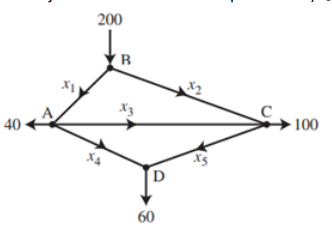
\includegraphics{image.png}
\caption{Alt text}
\end{figure}

\$\$ \begin{align*}
    200 = x_1 + x_2\\
    x_1 = 70 + x_3\\
    x_2 + X_3 = 100+25\\
    x_4 + x_5 = 60
\end{align*}

\rightarrow

\left[
    \begin{array}{rrrrr|r}
        1&1&0&0&0&200\\
        1&0&-&-1&0&40\\
        0&1&1&0&-1&100\\
        0&0&0&1&1&60
    \end{array}
\right]

\overrightarrow{
    \begin{align*}
        R_2 \rightarrow R_2 - R_1
    \end{align*}
} \textbackslash{}

\left[
    \begin{array}{rrrrr|r}
        1&1&0&0&0&200\\
        0&-1&-1&-1&0&-160\\
        0&1&1&0&-1&100\\
        0&0&0&1&1&60
    \end{array}
\right]

\overrightarrow{
    \begin{align*}
        R_2 \leftrightarrow R_3
    \end{align*}
}

\left[
    \begin{array}{rrrrr|r}
        1&1&0&0&0&200\\
        0&1&1&0&-1&100\\
        0&-1&-1&-1&0&-160\\
        0&0&0&1&1&60
    \end{array}
\right]

\overrightarrow{
    \begin{align*}
        R_1 \rightarrow R_1 \rightarrow R_2\\
        R_3 \rightarrow R_3 + R_2
    \end{align*}
} \textbackslash{}

\left[
    \begin{array}{rrrrr|r}
        1&0&-1&0&1&100\\
        0&1&1&0&-1&100\\
        0&0&0&-1&-1&-160\\
        0&0&0&1&1&60
    \end{array}
\right]

\overrightarrow{
    \begin{align*}
        R_3 \rightarrow -R_3
    \end{align*}
}

\left[
    \begin{array}{rrrrr|r}
        1&0&-1&0&1&100\\
        0&1&1&0&-1&100\\
        0&0&0&1&1&60\\
        0&0&0&1&1&60
    \end{array}
\right]

\overrightarrow{
    \begin{align*}
        R_4 \rightarrow R_4 - R_3
    \end{align*}
} \textbackslash{}

\left[
    \begin{array}{rrrrr|r}
        1&0&-1&0&1&100\\
        0&1&1&0&-1&100\\
        0&0&0&1&1&60\\
        0&0&0&0&0&0
    \end{array}
\right]\$\$

\[
x_1 = 100 + x_3 - x_5\\
x_2 = 100 - 2x_3 + x_5\\
x_4 = 60 - x_5\\
x_3 = x_3
x_5 = x_5
\]

Considerando la ecuación de \(x_1\), el valor mínimo de \(x_1\) es de
\(100\).

\hypertarget{use-las-leyes-de-kirchhoff-y-la-ley-de-ohm-para-establecer-un-sistema-de-ecuaciones-lineales-que-permita-determinar-las-corrientes-i_1-i_2-i_3-en-la-red-eluxe9ctrica-que-se-muestra-en-la-siguiente-figura.}{%
\paragraph{\texorpdfstring{33. Use las leyes de Kirchhoff y la ley de
Ohm para establecer un sistema de ecuaciones lineales que permita
determinar las corrientes \(I_1\), \(I_2\), \(I_3\) en la red eléctrica
que se muestra en la siguiente
figura.}{33. Use las leyes de Kirchhoff y la ley de Ohm para establecer un sistema de ecuaciones lineales que permita determinar las corrientes I\_1, I\_2, I\_3 en la red eléctrica que se muestra en la siguiente figura.}}\label{use-las-leyes-de-kirchhoff-y-la-ley-de-ohm-para-establecer-un-sistema-de-ecuaciones-lineales-que-permita-determinar-las-corrientes-i_1-i_2-i_3-en-la-red-eluxe9ctrica-que-se-muestra-en-la-siguiente-figura.}}

\begin{figure}
\centering
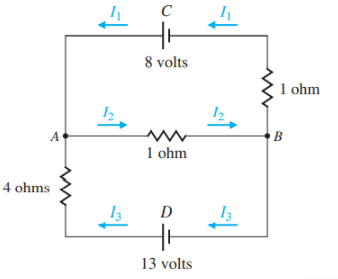
\includegraphics{image-1.png}
\caption{Alt text}
\end{figure}

\[
N_{eq} = 2 [LVK] + 0 [DS] + 0 [CS] = 2
\]

\[
LVK_1 = I_1 + I_2 - 8 = 0 \rightarrow I_1 + I_2 = 8\\
LVK_2 = -I_2 - 4I_3 + 13 = 0 \rightarrow -I_2 - 4I_3 = -13\\
\]

Soluciones:

\[
I_1 = 8 - I_2\\
I_2 = 13 - 4I_3\\
I_3 \in \R
\]

\hypertarget{considere-la-siguiente-reacciuxf3n-quuxedmica.-para-cada-uno-de-los-dos-reactivos-de-la-izquierda-y-los-cuatro-productos-de-la-derecha-construya-un-vector-en-ux211d5-que-liste-el-nuxfamero-de-uxe1tomos-por-moluxe9cula-de-plomo-pb-nitruxf3geno-n-cromo-cr-manganeso-mn-y-oxuxedgeno-o.-escriba-una-ecuaciuxf3n-vectorial-que-los-coeficientes-desconocidos-de-la-reacciuxf3n-deban-satisfacer-y-encuentre-una-soluciuxf3n-que-tenga-sentido-en-el-balance.}{%
\paragraph{34. Considere la siguiente reacción química. Para cada uno de
los dos reactivos de la izquierda y los cuatro productos de la derecha,
construya un vector en ℝ5 que liste el número de átomos por molécula de
plomo (Pb), nitrógeno (N), cromo (Cr), manganeso (Mn) y oxígeno (O).
Escriba una ecuación vectorial, que los coeficientes desconocidos de la
reacción deban satisfacer, y encuentre una solución que tenga sentido en
el
balance.}\label{considere-la-siguiente-reacciuxf3n-quuxedmica.-para-cada-uno-de-los-dos-reactivos-de-la-izquierda-y-los-cuatro-productos-de-la-derecha-construya-un-vector-en-ux211d5-que-liste-el-nuxfamero-de-uxe1tomos-por-moluxe9cula-de-plomo-pb-nitruxf3geno-n-cromo-cr-manganeso-mn-y-oxuxedgeno-o.-escriba-una-ecuaciuxf3n-vectorial-que-los-coeficientes-desconocidos-de-la-reacciuxf3n-deban-satisfacer-y-encuentre-una-soluciuxf3n-que-tenga-sentido-en-el-balance.}}

\[
PbN_6 + CrMn_2O_8 \rightarrow Pb_3O_4 + Cr_2O_3 + MnO_2 + NO
\]

Reactivos:

\$\$

\begin{align*}

    PbN = \begin{bmatrix}
        1&6&0&0&0
    \end{bmatrix} \\

    CrMnO = \begin{bmatrix}
        0&0&1&2&8
    \end{bmatrix} \\

    PbO = \begin{bmatrix}
        3&0&0&0&4
    \end{bmatrix} \\

    CrO = \begin{bmatrix}
        0&0&2&0&3
    \end{bmatrix} \\

    MnO = \begin{bmatrix}
        0&0&0&1&2
    \end{bmatrix} \\

    NO = \begin{bmatrix}
        0&1&0&0&1
    \end{bmatrix}

\end{align*}

\rightarrow

\left[
    \begin{array}{rrrrrr|r}
        1&0&-3&0&0&0&0\\
        6&0&0&0&0&-1&0\\
        0&1&0&-2&0&0&0\\
        0&2&0&0&-1&0&0\\
        0&8&-4&-3&-2&-1&0
    \end{array}
\right]

\overrightarrow{
    \begin{align*}
        R_2 \rightarrow R_2 - 6R_1
    \end{align*}
}

\textbackslash{}

\left[
    \begin{array}{rrrrrr|r}
        1&0&3&0&0&0&0\\
        0&0&18&0&0&-1&0\\
        0&1&0&-2&0&0&0\\
        0&2&0&0&-1&0&0\\
        0&8&-4&-3&-2&-1&0
    \end{array}
\right]

\overrightarrow{
    \begin{align*}
        R_3 \leftrightarrow R_2
    \end{align*}
}

\left[
    \begin{array}{rrrrrr|r}
        1&0&3&0&0&0&0\\
        0&1&0&-2&0&0&0\\
        0&0&18&0&0&-1&0\\
        0&2&0&0&-1&0&0\\
        0&8&-4&-3&-2&-1&0
    \end{array}
\right]

\overrightarrow{
    \begin{align*}
        R_4 \rightarrow R_4 - 2R_2\\
        R_5 \rightarrow R_5 - 8R-2
    \end{align*}
} \textbackslash{}

\left[
    \begin{array}{rrrrrr|r}
        1&0&3&0&0&0&0\\
        0&1&0&-2&0&0&0\\
        0&0&18&0&0&-1&0\\
        0&0&0&4&-1&0&0\\
        0&0&-4&-3&-2&-1&0
    \end{array}
\right]

\overrightarrow{
    \begin{align*}
        R_3 \rightarrow \frac{1}{18}R_3
    \end{align*}
}

\left[
    \begin{array}{rrrrrr|r}
        1&0&0&0&0&\frac{3}{18}&0\\
        0&1&0&-2&0&0&0\\
        0&0&1&0&0&-\frac{1}{18}&0\\
        0&0&0&4&-1&0&0\\
        0&0&0&13&-2&-\frac{11}{9}&0
    \end{array}
\right]

\overrightarrow{
    \begin{align*}
        R_4 \rightarrow \frac{1}{4}R_4
    \end{align*}
}

\textbackslash{}

\left[
    \begin{array}{rrrrrr|r}
        1&0&0&0&0&\frac{3}{18}&0\\
        0&1&0&-2&0&0&0\\
        0&0&1&0&0&-\frac{1}{18}&0\\
        0&0&0&1&-1&-\frac{1}{4}&0\\
        0&0&0&13&-2&-\frac{11}{9}&0
    \end{array}
\right]

\overrightarrow{
    \begin{align*}
        R_2 \rightarrow R_2 + 2R_4\\
        R_5 \rightarrow R_5 - 13R_4
    \end{align*}
}

\left[
    \begin{array}{rrrrrr|r}
        1&0&0&0&0&\frac{3}{18}&0\\
        0&1&0&-2&0&0&0\\
        0&0&1&0&0&-\frac{1}{18}&0\\
        0&0&0&1&-1&0&0\\
        0&0&0&0&-15&-\frac{11}{9}&0
    \end{array}
\right]

\overrightarrow{
    \begin{align*}
        R_5 \rightarrow -\frac{1}{15}R_5
    \end{align*}
} \textbackslash{}

\left[
    \begin{array}{rrrrrr|r}
        1&0&0&0&0&\frac{3}{18}&0\\
        0&1&0&0&-2&0&0\\
        0&0&1&0&0&-\frac{1}{18}&0\\
        0&0&0&1&-1&0&0\\
        0&0&0&0&1&-\frac{11}{135}&0
    \end{array}
\right]

\overrightarrow{
    \begin{align*}
        R_4 \rightarrow R_4 - R_5\\
        R_2 \rightarrow R_2 + 2R_5
    \end{align*}
}

\left[
    \begin{array}{rrrrrr|r}
        1&0&0&0&0&\frac{1}{6}&0\\
        0&1&0&0&0&\frac{22}{135}&0\\
        0&0&1&0&0&-\frac{1}{18}&0\\
        0&0&0&1&0&\frac{11}{135}&0\\
        0&0&0&0&1&-\frac{11}{135}&0
    \end{array}
\right]

\overrightarrow{
    \begin{align*}
        R_4 \rightarrow R_4 - R_5\\
        R_2 \rightarrow R_2 + 2R_5
    \end{align*}
} \textbackslash{}

\begin{align*}
    EC_1 = \frac{1}{6}EC_6
    EC_2 = \frac{22}{135}EC_6
    EC_3 = -\frac{1}{18}EC_6
    EC_4 = \frac{11}{135}EC_6
    EC_5 = \frac{11}{135}EC_6
\end{align*}

\$\$

\end{document}
